%% =====================================================================
%% HICA-S, Track T4 -- main results with proofs (reader-friendly version)
%% Section 1 is self-contained and is meant to be lifted into the journal
%% manuscript (COR).  Section 2 collects remarks, algorithms and the
%% computational evidence.  Numbers in Section 2 are taken from the
%% manuscript draft of 2026-09-30 and from the T4 audit reports.
%% Lines marked "% VERIFY" must be checked before submission.
%% =====================================================================
\documentclass[11pt]{article}
\usepackage[margin=2.4cm]{geometry}
\usepackage[T1]{fontenc}
\usepackage{lmodern}
\usepackage{microtype}
\usepackage{amsmath,amssymb,amsthm,mathtools}
\usepackage{booktabs,array,enumitem}
\usepackage{xcolor}
\usepackage{tikz}
\usetikzlibrary{arrows.meta,positioning,calc,decorations.pathreplacing,patterns,fit,backgrounds}
\usepackage{pgfplots}
\pgfplotsset{compat=1.18}
\usepackage{caption}
\usepackage{subcaption}
\usepackage{placeins}
\usepackage{algorithm}
\usepackage{algpseudocode}
\usepackage[authoryear,round]{natbib}
\usepackage[colorlinks=true,linkcolor=blue!50!black,citecolor=blue!50!black,urlcolor=blue!50!black]{hyperref}
\usepackage[capitalise,nameinlink]{cleveref}

\captionsetup{font=small,labelfont=bf}
\floatname{algorithm}{Procedure}
\algrenewcommand\algorithmicrequire{\textbf{Input:}}
\algrenewcommand\algorithmicensure{\textbf{Output:}}

% ---------------------------------------------------------------------
% Theorem-like environments
% ---------------------------------------------------------------------
\newtheorem{theorem}{Theorem}
\newtheorem{lemma}{Lemma}
\newtheorem{plemma}{Lemma}
\renewcommand{\theplemma}{P\arabic{plemma}}
\newtheorem{proposition}{Proposition}
\newtheorem{corollary}{Corollary}
\theoremstyle{definition}
\newtheorem{definition}{Definition}
\newtheorem{assumption}{Assumption}
\renewcommand{\theassumption}{A\arabic{assumption}}
\newtheorem*{standing}{Standing assumptions}
\newtheorem{example}{Example}
\theoremstyle{remark}
\newtheorem{remark}{Remark}

\crefname{plemma}{Lemma}{Lemmas}
\crefname{assumption}{Assumption}{Assumptions}
\crefname{algorithm}{Procedure}{Procedures}

% ---------------------------------------------------------------------
% Notation
% ---------------------------------------------------------------------
\newcommand{\Ks}{\mathcal{K}^{\star}}
\newcommand{\thl}{\underline{\theta}}
\newcommand{\thu}{\overline{\theta}}
\newcommand{\idle}{\mathbf{0}}
\newcommand{\FD}{\mathrm{FD}}
\newcommand{\pair}{\operatorname{pair}}
\newcommand{\R}{\mathbb{R}}
\DeclareMathOperator*{\argmin}{arg\,min}

% TikZ styles
\tikzset{
  box/.style={rectangle, rounded corners=2pt, draw=black!70, fill=#1, align=center,
              text width=3.3cm, minimum height=1.05cm, font=\footnotesize, inner sep=3pt},
  box/.default={gray!8},
  arr/.style={-{Stealth[length=2.2mm]}, thick, black!65},
  stop/.style={circle, fill=black, inner sep=1.4pt},
  order/.style={circle, fill=black!75, inner sep=1.2pt},
}

\title{HICA-S, Track T4: Local Pruning of Bid-Independent Route Pools\\[3pt]
\large Main results with complete proofs (reader-friendly version)}
\author{Tran An Khoa\\ \small Draft for supervisor review}
\date{October 2026}

\begin{document}
\maketitle

% =====================================================================
\section*{How to read this note}
% =====================================================================

The procurement mechanism of HICA-S generates a route pool for every driver
\emph{before} any bid is observed, and then runs exact VCG on that pool. This
note asks how far such a pool can be reduced, before bidding, by a rule that
looks only at the driver whose routes are being deleted.

\Cref{sec:main} is self-contained. It lists the notation (\cref{tab:notation}),
collects the elementary facts that are used repeatedly (\cref{sec:prelim}), and
then states and proves the three main results. In plain words:

\begin{itemize}[leftmargin=1.4em, itemsep=2pt]
\item \textbf{Theorem 1 (local pruning frontier).} A route $r$ of driver $i$
can be deleted safely, using only driver~$i$'s own data, exactly when for every
admissible report a \emph{local substitute} is at least as cheap: a route of
the same driver that serves part of the orders of $r$, with the remaining
orders sent to the fixed fleet (FD). Deleting all such routes changes no
optimal value and no VCG payment, and every route that survives is needed in
some instance, so no rule of this type can delete more.
\item \textbf{Theorem 2 (price of locality).} The surviving pool can still
contain one route for each of the $\Theta(n^B)$ bundles of at most $B$ orders,
even in instances in which none of these routes is ever used.
\item \textbf{Theorem 3 (label rule).} Part of the test can be carried out
while routes are being generated, so that partial routes are discarded early,
without changing the surviving pool.
\end{itemize}

\Cref{sec:remarks} contains remarks, the procedures that compute these objects,
the NP-hardness of exact non-local pruning, and the computational evidence.
Nothing in \cref{sec:main} depends on \cref{sec:remarks}. \Cref{fig:roadmap}
shows how the results depend on each other.

\begin{figure}[!htbp]
\centering
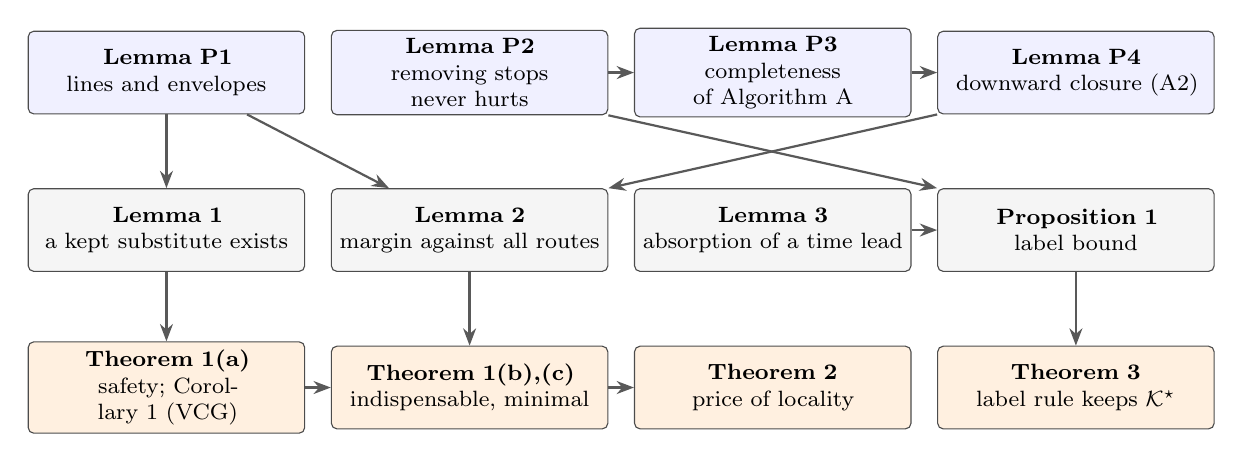
\begin{tikzpicture}[x=1cm,y=1cm]
\node[box=blue!6]  (P1) at (0,0)    {\textbf{Lemma P1}\\ lines and envelopes};
\node[box=blue!6]  (P2) at (3.85,0) {\textbf{Lemma P2}\\ removing stops never hurts};
\node[box=blue!6]  (P3) at (7.7,0)  {\textbf{Lemma P3}\\ completeness of Algorithm~A};
\node[box=blue!6]  (P4) at (11.55,0){\textbf{Lemma P4}\\ downward closure (A2)};
\node[box]         (L1) at (0,-2)   {\textbf{Lemma 1}\\ a kept substitute exists};
\node[box]         (L2) at (3.85,-2){\textbf{Lemma 2}\\ margin against all routes};
\node[box]         (L3) at (7.7,-2) {\textbf{Lemma 3}\\ absorption of a time lead};
\node[box]         (Q1) at (11.55,-2){\textbf{Proposition 1}\\ label bound};
\node[box=orange!12] (T1a) at (0,-4)   {\textbf{Theorem 1(a)}\\ safety; Corollary 1 (VCG)};
\node[box=orange!12] (T1b) at (3.85,-4){\textbf{Theorem 1(b),(c)}\\ indispensable, minimal};
\node[box=orange!12] (T2)  at (7.7,-4) {\textbf{Theorem 2}\\ price of locality};
\node[box=orange!12] (T3)  at (11.55,-4){\textbf{Theorem 3}\\ label rule keeps $\Ks$};
\draw[arr] (P1) -- (L1);
\draw[arr] (P1) -- (L2);
\draw[arr] (P4.south west) -- (L2.north east);
\draw[arr] (P2) -- (P3);
\draw[arr] (P3) -- (P4);
\draw[arr] (L1) -- (T1a);
\draw[arr] (L2) -- (T1b);
\draw[arr] (T1a) -- (T1b);
\draw[arr] (T1b) -- (T2);
\draw[arr] (L3) -- (Q1);
\draw[arr] (P2.south east) -- (Q1.north west);
\draw[arr] (Q1) -- (T3);
\end{tikzpicture}
\caption{Roadmap. Blue boxes are preliminaries (\cref{sec:prelim}), white boxes
are the lemmas behind the main results, orange boxes are the main results.
Theorem~3 also uses Lemma~1 and Lemma~P3.}
\label{fig:roadmap}
\end{figure}

% =====================================================================
\section{Main results}
\label{sec:main}
% =====================================================================

\subsection{Setting and notation}
\label{sec:setting}

\paragraph{Orders and the fixed fleet.}
$O$ is a finite set of orders. Every order $o\in O$ can always be delegated to
the fixed-capacity fleet (FD) at a public price $q_o\ge 0$; for $A\subseteq O$
we write $q(A):=\sum_{o\in A}q_o$. The platform publishes a bundle cap $B\ge1$.

\paragraph{Drivers, routes and costs.}
$N$ is the set of strategic drivers (gigworkers and occasional drivers). Driver
$i$ owns a finite route pool $R_i$, fixed before reports are collected. A route
$r\in R_i$ serves a nonempty \emph{bundle} $S_r\subseteq O$ with $|S_r|\le B$
and has two public nonnegative coefficients, its \emph{pair}
$\pair(r)=(K_r,W_r)$: $K_r$ is a distance cost and $W_r$ is working time in
hours. If the driver reports the value of time $b\ge 0$, the reported cost of
$r$ is
\begin{equation}\label{eq:cost}
  c_r(b)\;=\;K_r+b\,W_r .
\end{equation}
Thus every route is a \emph{line} in the report $b$, with intercept $K_r$ and
slope $W_r$. The idle option of driver $i$ is the empty route $\idle_i$ with
$S_{\idle_i}=\emptyset$ and $K=W=0$. We write
$\pair(r)\le\pair(r')$ if $K_r\le K_{r'}$ and $W_r\le W_{r'}$; then
$c_r(b)\le c_{r'}(b)$ for every $b\ge0$.

\paragraph{Reports and the pruning domain.}
Pruning is required to be correct for all report profiles in a domain
$\Theta=[\thl,\thu]$ with $0\le\thl<\thu$, announced before bidding (in the
experiments $\Theta=[18,25]$ money units per hour).

\paragraph{Winner determination and payments.}
An \emph{allocation} $\rho=(\rho_j)_{j\in N}$ assigns to every driver one route
$\rho_j\in R_j\cup\{\idle_j\}$ such that the bundles are pairwise disjoint;
orders that no selected route serves are sent to FD. For a report profile
$b=(b_j)_{j\in N}$ its cost is
\begin{equation}\label{eq:alloccost}
C(\rho;b)\;=\;\sum_{j\in N}c_{\rho_j}(b_j)\;+\;q\Bigl(O\setminus\bigcup_{j\in N}S_{\rho_j}\Bigr).
\end{equation}
$V(R;b)$ is the minimum of $C(\rho;b)$ over all allocations; this is the
set-partitioning winner-determination problem (Algorithm~B), in which every
order is served exactly once, by a route or by FD, and every driver receives at
most one route. $V_{-k}(R;b)$ is the same minimum with driver $k$ removed
(Algorithm~C). A winner $k$ with route $\rho^*_k$ is paid the Clarke-pivot
payment
\begin{equation}\label{eq:payment}
p_k\;=\;c_{\rho^*_k}(b_k)+V_{-k}(R;b)-V(R;b).
\end{equation}
For sub-pools $R'_j\subseteq R_j$ we write $V(R';b)$ for the same problem on
the smaller pools.

\paragraph{Routes as stop sequences.}
Only the proofs of \cref{lem:remove,lem:complete,lem:downward} and of
Theorems~2 and~3 look inside a route. There, a route of driver $i$ is a
sequence of stops (pickup $p_o$ and delivery $d_o$ of each served order)
starting from the point $v_0$ at the fixed departure time $t_0$. At its
$k$-th stop $v_k$ the driver starts service and becomes ready to leave at
\begin{equation}\label{eq:recursion}
a_k=\max\bigl\{e_{v_k},\;r_{k-1}+\tau(v_{k-1},v_k)\bigr\},\qquad
r_k=a_k+s_{v_k},\qquad r_0=t_0,
\end{equation}
where $\tau$ is travel time (minutes), $s_v$ the service time and $e_v$ the
opening time of stop $v$ (the release time for a pickup; $e_v=-\infty$ if the
stop has no opening time). The $\max$ in \eqref{eq:recursion} is the waiting
time: a driver who arrives before $e_v$ waits.

\begin{standing}
The following conditions hold throughout.
\begin{enumerate}[label=(S\arabic*), leftmargin=2.6em, itemsep=1pt]
\item Distances $d(\cdot,\cdot)$ and travel times $\tau(\cdot,\cdot)$ are
nonnegative and satisfy the triangle inequality; service times are nonnegative.
\item Opening and release times are lower bounds, met by waiting. Closing
times, the end of availability, the capacity, the bundle cap $B$ and (for an
occasional driver) the detour budget are upper bounds.
\item For a gigworker with distance coefficient $\kappa$,
$K=\kappa\cdot(\text{route length})$ and $W=(\text{completion time}-t_0)/60$.
For an occasional driver the route ends at her personal destination and
$K=\kappa\cdot(\text{route length}-\text{direct length})$,
$W=(\text{arrival time}-t_0-\text{direct time})/60$; both are nonnegative by
(S1).
\end{enumerate}
\end{standing}

\Cref{tab:notation} lists all symbols used in \cref{sec:main}.

\begin{table}[!htbp]
\centering
\caption{Notation.}
\label{tab:notation}
\small
\renewcommand{\arraystretch}{1.12}
\begin{tabular}{@{}>{$}l<{$}p{12.2cm}@{}}
\toprule
\multicolumn{2}{@{}l}{\textit{Data}}\\
O;\; o,j,x & set of orders; generic orders\\
q_o,\; q(A) & FD price of order $o$; $q(A)=\sum_{o\in A}q_o$\\
B & bundle cap: a route serves at most $B$ orders\\
N & set of strategic drivers (gigworkers and occasional drivers)\\
\Theta=[\thl,\thu] & pruning domain of reports, announced before bidding, $0\le\thl<\thu$\\
b_i;\; b=(b_i)_{i\in N} & report of driver $i$ (value of time, per hour); report profile\\
\midrule
\multicolumn{2}{@{}l}{\textit{Routes and costs}}\\
R_i & route pool of driver $i$, fixed before reports\\
\idle_i & idle route of driver $i$: no orders, $K=W=0$\\
S_r & bundle of route $r$ (set of orders it serves), $1\le|S_r|\le B$\\
\pair(r)=(K_r,W_r) & distance cost and working time (hours) of $r$\\
c_r(b)=K_r+bW_r & reported cost of $r$; a line in $b$ with intercept $K_r$, slope $W_r$\\
\pair(r)\le\pair(r') & $K_r\le K_{r'}$ and $W_r\le W_{r'}$; implies $c_r(b)\le c_{r'}(b)$ for all $b\ge0$\\
\midrule
\multicolumn{2}{@{}l}{\textit{Allocation and payments}}\\
\rho=(\rho_j)_{j\in N} & allocation: one route or $\idle_j$ per driver, disjoint bundles, the rest to FD\\
C(\rho;b) & cost \eqref{eq:alloccost} of allocation $\rho$ at reports $b$\\
V(R;b),\; V_{-k}(R;b) & optimal value; optimal value without driver $k$\\
p_k & Clarke-pivot payment \eqref{eq:payment}\\
\midrule
\multicolumn{2}{@{}l}{\textit{Local frontier (\cref{sec:frontier})}}\\
L_i=(O,q,B,\Theta,R_i) & local view of driver $i$: everything a local rule may read\\
D(r) & local substitutes of $r$: other routes of the same driver serving a subset of $S_r$, and $\idle_i$\\
g_{r'}(b) & substitute line $c_{r'}(b)+q(S_r\setminus S_{r'})$: use $r'$, send the rest of $S_r$ to FD\\
E_r(b) & FD-completion envelope: the lowest substitute line at $b$\\
\mu_r(b)=E_r(b)-c_r(b) & local margin of $r$: how much $r$ saves over its best local substitute\\
\Ks_i & local frontier of driver $i$: routes with $\mu_r(b)>0$ for some $b\in\Theta$\\
\Pi^\star & frontier rule: delete $R_i\setminus\Ks_i$ for every driver\\
\midrule
\multicolumn{2}{@{}l}{\textit{Routing (Lemmas P2--P4, Theorems 2--3)}}\\
p_o,\; d_o & pickup and delivery stop of order $o$\\
v_0,\; t_0 & start point and (fixed) departure time of a driver\\
d(u,v),\;\tau(u,v) & distance (km) and travel time (min) from $u$ to $v$\\
s_v,\; e_v,\; l_v & service time, opening time and closing time of stop $v$\\
a_k,\; r_k & service start and ready time at the $k$-th stop, \eqref{eq:recursion}\\
\kappa & distance coefficient (money per km)\\
L,\; P(L) & label (a partial route) and the set of orders picked up in it\\
\Delta D,\;\delta,\;A,\;\beta & distance spent on $T$, time spent on $T$, absorption term, label bound (\cref{def:shortcut})\\
\bottomrule
\end{tabular}
\end{table}

% ---------------------------------------------------------------------
\subsection{Preliminaries}
\label{sec:prelim}
% ---------------------------------------------------------------------

\paragraph{Lines and lower envelopes.}
Because every cost \eqref{eq:cost} is a line in the report, the whole analysis
reduces to comparing lines on an interval. The following facts are elementary
and are used without further comment.

\begin{plemma}[Lines and lower envelopes]\label{lem:lines}
Let $g_1,\dots,g_m$ be lines in $b$ and $E(b)=\min_j g_j(b)$ their lower
envelope (\cref{fig:envelope}a).
\begin{enumerate}[label=(\roman*), itemsep=1pt]
\item $E$ is continuous, concave and piecewise linear. Its \emph{breakpoints}
are the values of $b$ at which the lowest line changes.
\item For any further line $c$, the difference $E-c$ is concave and piecewise
linear with the same breakpoints. On an interval $[\thl,\thu]$ its maximum is
attained at $\thl$, at $\thu$ or at a breakpoint in between.
\item Two different lines agree at no more than one point. Hence a line that is
nonnegative on an interval of positive length and is not identically zero is
strictly positive on that interval except at, at most, one point.
\item If finitely many strict inequalities between lines hold at $b$, they
also hold at every $b'$ close enough to $b$.
\end{enumerate}
\end{plemma}

\begin{proof}
A minimum of affine functions is concave; between two consecutive breakpoints
$E-c$ is affine, so its maximum over each piece is at an end of the piece. The
difference of two different lines is a nonzero affine function and has at most
one root. Item (iv) is continuity.
\end{proof}

\paragraph{Removing stops.}
The next lemma is the only place where routing enters the theory. Shortening a
route obviously shortens its length; that it also never delays a later stop is
less obvious, because a driver who arrives earlier may simply wait longer.

\begin{plemma}[Removing stops never hurts]\label{lem:remove}
Let $\sigma'$ be obtained from a stop sequence $\sigma$ by deleting some
stops, both starting at $(v_0,t_0)$. Under (S1)--(S2):
\begin{enumerate}[label=(\roman*), itemsep=1pt]
\item $\sigma'$ is no longer than $\sigma$;
\item every stop kept in $\sigma'$ starts service in $\sigma'$ no later than in
$\sigma$;
\item the completion time (for an occasional driver, the arrival time at the
destination) of $\sigma'$ is no later than that of $\sigma$.
\end{enumerate}
Neither sequence needs to be feasible.
\end{plemma}

\begin{proof}
(i) is the triangle inequality, applied to every stretch of deleted stops.
(ii) Let $u$ and $v$ be consecutive kept stops. In $\sigma$ the driver travels
from $u$ to $v$ through deleted stops, so, since waiting and service are
nonnegative and by the triangle inequality,
$a_\sigma(v)\ge a_\sigma(u)+s_u+\tau(u,v)$; moreover $a_\sigma(v)\ge e_v$. In
$\sigma'$, by \eqref{eq:recursion},
$a_{\sigma'}(v)=\max\{e_v,\,a_{\sigma'}(u)+s_u+\tau(u,v)\}$. Hence
$a_{\sigma'}(u)\le a_\sigma(u)$ implies $a_{\sigma'}(v)\le a_\sigma(v)$. The
first kept stop is treated in the same way with $u=v_0$, and induction gives
(ii). (iii) follows from (ii) applied to the last stop, or to the destination
regarded as a final stop without opening time.
\end{proof}

\paragraph{Algorithm A.}
Algorithm~A generates the pool of each driver by forward label setting. A
\emph{label} is a partial route, stored as $(v,IV,C,t,K,W)$: current stop,
orders on board, orders delivered, clock, and accumulated costs. Labels are
extended one stop at a time and pass three filters (\cref{alg:routegen} in
\cref{sec:remarks}):
\begin{itemize}[leftmargin=1.4em, itemsep=1pt]
\item \emph{Layer 1 (label dominance).} Labels are processed in
\emph{batches}. Within a batch, a label is removed if another label with the
same key $(v,IV,C)$ has no later clock and no larger $K$ and $W$, one of them
strictly smaller. Every label that is created is filtered in exactly one batch,
and its extensions are filtered in later batches.
\item \emph{Layer 2 (per-bundle Pareto).} Among completed routes with the same
bundle, only the Pareto-minimal pairs $(K,W)$ are kept, one route per pair.
\item \emph{Layer 3 (optional label rule).} The rule of \cref{sec:label}.
\end{itemize}
The returned pool $R_i$ therefore contains no two routes with the same bundle
and the same pair.

\begin{plemma}[Completeness of Algorithm A]\label{lem:complete}
Let $\rho$ be any feasible route of driver $i$ and $R_i$ the pool returned by
Algorithm~A, possibly with Layer~3 switched on. Then
\begin{enumerate}[label=(\alph*), itemsep=1pt]
\item $R_i$ contains a route with bundle $S_\rho$ and pair at most $\pair(\rho)$; or
\item some feasible route $\tilde\rho$ with $S_{\tilde\rho}=S_\rho$ and
$\pair(\tilde\rho)\le\pair(\rho)$ passes through a label discarded by Layer~3.
\end{enumerate}
Alternative (b) is impossible without Layer~3. In that case $R_i$ contains
exactly one route for each Pareto-minimal pair of each bundle.
\end{plemma}

\begin{proof}
Follow the prefixes of $\rho$ (the labels it passes through) during the run,
and look at the first prefix that does not survive.

\emph{Case 1: every prefix survives.} Then $\rho$ is completed, and Layer~2
keeps a route with bundle $S_\rho$ and pair at most $\pair(\rho)$: (a) holds.

\emph{Case 2: a prefix is discarded by Layer~3.} Then (b) holds with
$\tilde\rho=\rho$.

\emph{Case 3: a prefix $L$ is removed by Layer~1.} Dominance is irreflexive and
transitive, so in the finite batch of $L$ some label $L'$ that dominates $L$
survives. $L'$ is at the same stop, has the same orders on board and the same
orders delivered, and has no later clock and no larger costs. Append the
remaining stops of $\rho$ to $L'$. By \eqref{eq:recursion}, starting earlier
never makes a later service start later, so every remaining stop is served no
later than in $\rho$ and all closing times are met. The added distance is the
same and the completion (or arrival) time is no later, so the result is a
feasible route $\rho'$ with $S_{\rho'}=S_\rho$ and $\pair(\rho')\le\pair(\rho)$. All prefixes of
$\rho'$ up to $L'$ survive. Repeat the argument with $\rho'$ in place of $\rho$:
its first non-surviving prefix lies in a strictly later batch. As there are
finitely many batches, Case~1 or Case~2 is eventually reached for some route
whose pair is at most $\pair(\rho)$, and (a) or (b) follows for $\rho$.

Without Layer~3, Case~2 never occurs, so (a) holds for every feasible route. A
route kept by Layer~2 cannot be dominated by a feasible route $\rho''$ of the
same bundle, because (a) for $\rho''$ would produce a kept route dominating it.
Conversely, for a Pareto-minimal pair, (a) produces a kept route with exactly
that pair.
\end{proof}

\paragraph{Downward closure.}
The next property says that taking orders out of a route never makes it more
expensive (\cref{fig:downward}). It is assumption~A2 below, and it holds
automatically for the pools of Algorithm~A.

\begin{plemma}[Pools of Algorithm A are downward closed]\label{lem:downward}
Let $R_i$ be produced by Algorithm~A without Layer~3. For every $r'\in R_i$ and
every $T\subseteq S_{r'}$ there is $\hat r\in R_i\cup\{\idle_i\}$ with
$S_{\hat r}=T$ and $\pair(\hat r)\le\pair(r')$.
\end{plemma}

\begin{proof}
For $T=\emptyset$ take $\hat r=\idle_i$. Otherwise delete from $r'$ the pickup
and delivery of every order outside $T$, and call the result $\sigma$. By
\cref{lem:remove}, $\sigma$ is no longer than $r'$ and serves every remaining
stop no later; hence closing times, availability and (for an occasional driver)
the detour budget are respected. The load at each remaining stop is that of the
orders of $T$ on board, which is at most the original load; precedence is
inherited, and $|T|\le B$. So $\sigma$ is feasible, and $\pair(\sigma)\le\pair(r')$
because both its length and its completion (or arrival) time are no larger.
\Cref{lem:complete} without Layer~3 gives a route $\hat r\in R_i$ with bundle
$T$ and $\pair(\hat r)\le\pair(\sigma)\le\pair(r')$.
\end{proof}

\begin{figure}[!htbp]
\centering
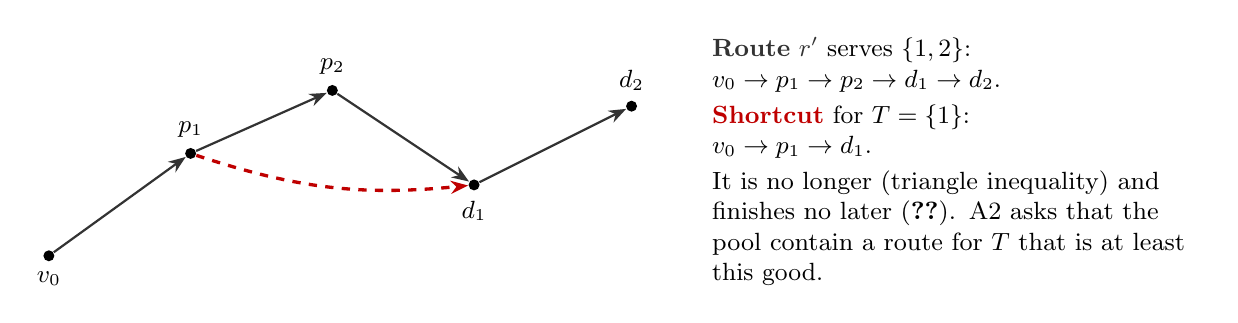
\begin{tikzpicture}[x=1cm,y=1cm, font=\small]
\node[stop, label=below:{$v_0$}] (v0) at (0,0) {};
\node[stop, label=above:{$p_1$}] (p1) at (1.8,1.3) {};
\node[stop, label=above:{$p_2$}] (p2) at (3.6,2.1) {};
\node[stop, label=below:{$d_1$}] (d1) at (5.4,0.9) {};
\node[stop, label=above:{$d_2$}] (d2) at (7.4,1.9) {};
\draw[arr, black!80] (v0) -- (p1);
\draw[arr, black!80] (p1) -- (p2);
\draw[arr, black!80] (p2) -- (d1);
\draw[arr, black!80] (d1) -- (d2);
\draw[arr, red!75!black, dashed, very thick] (p1) to[bend right=12] (d1);
\node[align=left, anchor=west, text width=6.2cm] at (8.3,1.2)
{\textcolor{black!80}{\textbf{Route $r'$}} serves $\{1,2\}$:\\ $v_0\to p_1\to p_2\to d_1\to d_2$.\\[2pt]
\textcolor{red!75!black}{\textbf{Shortcut}} for $T=\{1\}$:\\ $v_0\to p_1\to d_1$.\\[2pt]
It is no longer (triangle inequality) and finishes no later (\cref{lem:remove}).
A2 asks that the pool contain a route for $T$ that is at least this good.};
\end{tikzpicture}
\caption{Downward closure (Assumption~A2, \cref{lem:downward}): deleting the
stops of some orders from a feasible route gives a feasible route for the
remaining orders whose distance cost and working time are both no larger.}
\label{fig:downward}
\end{figure}

\paragraph{Truthfulness.}
The mechanism itself is exact VCG on a range that is fixed before bidding; its
incentive properties are classical.

\begin{plemma}[Truthfulness; \citealp{nisan2007computationally}]\label{lem:dsic}
If the pools are fixed before reports are observed, every base and removal
problem is solved exactly, ties are broken by a rule that reads no report, and
costs have the form \eqref{eq:cost}, then truthful reporting is a dominant
strategy and every driver's utility is nonnegative.
\end{plemma}

\begin{proof}
This is the maximal-in-range argument: the utility of driver $i$ equals
$V_{-i}(R;b)$ minus the cost of the selected allocation evaluated at $i$'s true
cost and the others' reports, and the mechanism minimises exactly that cost
when $i$ reports truthfully. Utility is nonnegative because $\idle_i$ is always
available. See \citet{nisan2007computationally}.
\end{proof}

% ---------------------------------------------------------------------
\subsection{The local frontier}
\label{sec:frontier}
% ---------------------------------------------------------------------

\begin{definition}[Local view, local rule, safety]\label{def:local}
The \emph{local view} of driver $i$ is $L_i=(O,q,B,\Theta,R_i)$. A
\emph{local pruning rule} $\Pi$ is a deterministic map that assigns to every
local view a set $\Pi(L_i)\subseteq R_i$ of routes to delete; applied to every
driver it yields the pools $R^\Pi_j=R_j\setminus\Pi(L_j)$. An \emph{instance}
is any finite set of drivers whose pools consist of routes with bundles of size
at most $B$ and nonnegative coefficients, in which no two routes of the same
driver share both the bundle and the pair. The rule is \emph{safe} if
$V(R^\Pi;b)=V(R;b)$ for every instance and every $b\in\Theta^N$.
\end{definition}

A local rule reads no report, so the pruned pools are fixed before bidding and
\cref{lem:dsic} still applies. The ban on duplicates is harmless: duplicates can
be merged before pruning without changing any optimal value, and Algorithm~A
never produces them.

\paragraph{Assumptions on the pool of the driver under study.}
Theorem~1(b)--(c) and Theorem~2 use the following three properties of a single
pool $R_i$.

\begin{assumption}[No duplicates]\label{ass:nodup}
No two routes of $R_i$ have the same bundle and the same pair.
\end{assumption}

\begin{assumption}[Downward closure: dropping orders never costs more]\label{ass:down}
For every route $r'\in R_i$ and every set $T\subseteq S_{r'}$ of its orders,
$R_i\cup\{\idle_i\}$ contains a route $\hat r$ with $S_{\hat r}=T$ and
$\pair(\hat r)\le\pair(r')$.
\end{assumption}

\begin{assumption}[No free extra orders]\label{ass:nofree}
If $r,r'\in R_i$ and $S_r\subsetneq S_{r'}$, then $\pair(r)\ne\pair(r')$:
serving additional orders costs some distance or some time.
\end{assumption}

\Cref{ass:nodup} holds in every instance by \cref{def:local};
\cref{ass:nodup,ass:down} hold for every pool of Algorithm~A by
\cref{lem:complete,lem:downward} (see \cref{fig:downward}).
\Cref{ass:nofree} only excludes serving extra orders at exactly zero extra
distance and zero extra time.

\paragraph{The envelope, the margin and the frontier.}
When the platform considers deleting a route $r$ of driver $i$ without looking
at other drivers, the only replacements it can trust are those that involve
nobody else: another route $r'$ of driver $i$ that serves \emph{part} of $S_r$,
with the remaining orders $S_r\setminus S_{r'}$ sent to FD at their public
price. At report $b$ such a replacement costs
$g_{r'}(b)=c_{r'}(b)+q(S_r\setminus S_{r'})$, again a line in $b$.

\begin{definition}[Substitutes, envelope, margin, frontier]\label{def:frontier}
For $r\in R_i$, the set of \emph{local substitutes} is
\[
D(r)=\bigl\{\,r'\in R_i\cup\{\idle_i\}:\ r'\ne r,\ S_{r'}\subseteq S_r\,\bigr\}.
\]
The \emph{FD-completion envelope} and the \emph{local margin} of $r$ are
\[
E_r(b)=\min_{r'\in D(r)}\bigl\{c_{r'}(b)+q(S_r\setminus S_{r'})\bigr\},
\qquad
\mu_r(b)=E_r(b)-c_r(b).
\]
The \emph{local frontier} of driver $i$ is
$\Ks_i=\{\,r\in R_i:\ \mu_r(b)>0\text{ for some }b\in\Theta\,\}$, and the
\emph{frontier rule} $\Pi^\star$ deletes $R_i\setminus\Ks_i$ for every driver.
\end{definition}

In words, $\mu_r(b)$ is how much route $r$ saves, at report $b$, compared with
the best way of doing without $r$ that uses only driver $i$ and FD. A route
belongs to the frontier if it is strictly the best local option for at least
one admissible report. Since $\idle_i\in D(r)$, always $E_r(b)\le q(S_r)$.
\Cref{fig:envelope} illustrates the definition. By \cref{lem:lines}(ii),
membership in $\Ks_i$ is decided by evaluating $\mu_r$ at $\thl$, at $\thu$ and
at the breakpoints of $E_r$ in between (\cref{alg:frontier}).

\begin{figure}[!htbp]
\centering
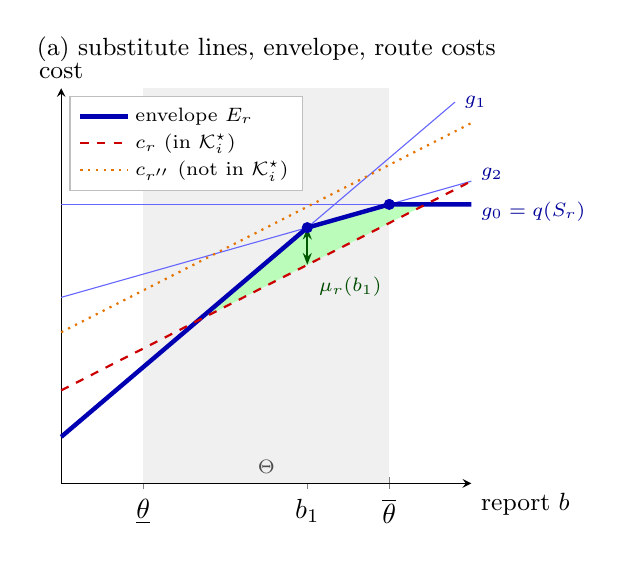
\begin{tikzpicture}
\begin{axis}[width=0.56\textwidth, height=6.6cm, xmin=0, xmax=10, ymin=0, ymax=17,
  axis lines=left, xlabel={report $b$}, ylabel={cost},
  xtick={2,6,8}, xticklabels={$\thl$,$b_1$,$\thu$}, ytick=\empty,
  clip=false, title={(a) substitute lines, envelope, route costs}, title style={font=\small},
  every axis x label/.style={at={(ticklabel* cs:1)}, anchor=north west, font=\small},
  every axis y label/.style={at={(ticklabel* cs:1)}, anchor=south, font=\small},
  legend style={at={(0.02,0.98)}, anchor=north west, font=\scriptsize, draw=gray!50, fill=white, row sep=-1pt},
  legend cell align=left]
\fill[gray!12] (axis cs:2,0) rectangle (axis cs:8,17);
\node[font=\scriptsize, gray!60!black] at (axis cs:5,0.7) {$\Theta$};
\fill[green!30, opacity=0.85] (axis cs:3.333,7) -- (axis cs:8.889,12) -- (axis cs:8,12) -- (axis cs:6,11) -- cycle;
\addplot[domain=0:9.6, thin, blue!60, forget plot] {2+1.5*x};
\addplot[domain=0:10, thin, blue!60, forget plot] {8+0.5*x};
\addplot[domain=0:10, thin, blue!60, forget plot] {12};
\addplot[domain=0:10, samples=201, ultra thick, blue!70!black] {min(2+1.5*x, 8+0.5*x, 12)};
\addlegendentry{envelope $E_r$}
\addplot[domain=0:10, thick, red!80!black, dashed] {4+0.9*x};
\addlegendentry{$c_r$ (in $\Ks_i$)}
\addplot[domain=0:10, thick, orange!90!black, dotted] {6.5+0.9*x};
\addlegendentry{$c_{r''}$ (not in $\Ks_i$)}
\addplot[only marks, mark=*, mark size=1.8pt, blue!70!black, forget plot] coordinates {(6,11) (8,12)};
\node[font=\scriptsize, blue!60!black, anchor=west] at (axis cs:9.6,16.4) {$g_1$};
\node[font=\scriptsize, blue!60!black, anchor=west] at (axis cs:10,13.3) {$g_2$};
\node[font=\scriptsize, blue!60!black, anchor=west] at (axis cs:10,11.7) {$g_0=q(S_r)$};
\draw[{Stealth[length=1.5mm]}-{Stealth[length=1.5mm]}, thick, green!35!black] (axis cs:6,9.4) -- (axis cs:6,11);
\node[font=\scriptsize, green!30!black, anchor=north west] at (axis cs:6.05,9.3) {$\mu_r(b_1)$};
\end{axis}
\end{tikzpicture}\hfill
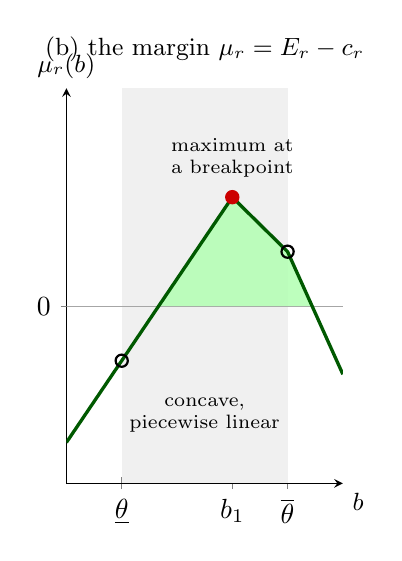
\begin{tikzpicture}
\begin{axis}[width=0.42\textwidth, height=6.6cm, xmin=0, xmax=10, ymin=-2.6, ymax=3.2,
  axis lines=left, xlabel={$b$}, ylabel={$\mu_r(b)$},
  xtick={2,6,8}, xticklabels={$\thl$,$b_1$,$\thu$}, ytick={0},
  title={(b) the margin $\mu_r=E_r-c_r$}, title style={font=\small},
  every axis x label/.style={at={(ticklabel* cs:1)}, anchor=north west, font=\small},
  every axis y label/.style={at={(ticklabel* cs:1)}, anchor=south, font=\small}]
\fill[gray!12] (axis cs:2,-2.6) rectangle (axis cs:8,3.2);
\draw[gray!70] (axis cs:0,0) -- (axis cs:10,0);
\fill[green!30, opacity=0.85] (axis cs:3.333,0) -- (axis cs:6,1.6) -- (axis cs:8,0.8) -- (axis cs:8.889,0) -- cycle;
\addplot[domain=0:10, samples=201, very thick, green!35!black] {min(2+1.5*x, 8+0.5*x, 12)-(4+0.9*x)};
\addplot[only marks, mark=o, mark size=2.2pt, thick, black] coordinates {(2,-0.8) (8,0.8)};
\addplot[only marks, mark=*, mark size=2.4pt, red!80!black] coordinates {(6,1.6)};
\node[font=\scriptsize, anchor=south, align=center] at (axis cs:6,1.75) {maximum at\\ a breakpoint};
\node[font=\scriptsize, anchor=north, align=center] at (axis cs:5,-1.2) {concave,\\ piecewise linear};
\end{axis}
\end{tikzpicture}
\caption{The envelope and the margin. (a) Each thin line is a local substitute
$g_{r'}(b)=c_{r'}(b)+q(S_r\setminus S_{r'})$; $g_0$ is the idle option (all of
$S_r$ to FD). The thick line is their lower envelope $E_r$, with breakpoints
(dots) where the lowest substitute changes. Route $r$ (dashed) lies below $E_r$
on the green region, so it is in the frontier. Route $r''$ (dotted) lies above
$E_r$ everywhere, so some local substitute is always at least as cheap and
$r''$ can be deleted. (b) The margin $\mu_r=E_r-c_r$ is concave and piecewise
linear, so its maximum over $\Theta$ is attained at $\thl$, at $\thu$ or at a
breakpoint (\cref{lem:lines}); here at the breakpoint $b_1$.}
\label{fig:envelope}
\end{figure}

\begin{example}[Twin instances]\label{ex:twin}
A gigworker $g$ faces two orders with $q_{o_1}=15$, $q_{o_2}=45$, and
$\Theta=[18,25]$. Her pool has three routes:
\[
r_a:\ \{o_1\},\ (6,0.6);\qquad r_b:\ \{o_2\},\ (8,0.8);\qquad r_c:\ \{o_1,o_2\},\ (11,1.2).
\]
\emph{Frontier.} $r_a$: its only substitute is $\idle_g$, so
$E_{r_a}=q_{o_1}=15<6+0.6b$ on $\Theta$; $r_a\notin\Ks_g$ (FD is always
cheaper). $r_b$: $E_{r_b}=45>8+0.8b$ on $\Theta$, so $r_b\in\Ks_g$. $r_c$: at
$b=18$ the three substitutes cost $6+10.8+45=61.8$ ($r_a$, $o_2$ to FD),
$8+14.4+15=37.4$ ($r_b$, $o_1$ to FD) and $60$ (idle), so
$E_{r_c}(18)=37.4>32.6=c_{r_c}(18)$ and $r_c\in\Ks_g$.

\emph{Instance $I_0$} ($g$ alone). $r_c$ costs less than $r_b$ plus FD for
$o_1$ iff $11+1.2b<23+0.8b$, i.e.\ $b<30$; so $r_c$ is optimal on all of
$\Theta$ and $r_b$ is never used.

\emph{Instance $I_1$} ($I_0$ plus a driver who serves $o_1$ at cost $0.5$). At
$b=18$ the optimum is $22.4+0.5=22.9$ and uses $r_b$; without $r_b$ it is
$32.6$.

A rule that deletes $r_b$ --- for instance a hull across bundles, under which
$r_a$ dominates $r_b$ --- is right on $I_0$ and wrong on $I_1$. Driver $g$'s
data cannot tell the two instances apart. This is Theorem~1(b) in its smallest
form.
\end{example}

% ---------------------------------------------------------------------
\subsection{Theorem 1: the local pruning frontier}
\label{sec:thm1}
% ---------------------------------------------------------------------

\begin{theorem}[Local pruning frontier]\label{thm:frontier}
Let $\thl<\thu$.
\begin{enumerate}[label=(\alph*), itemsep=2pt]
\item \textbf{Safety.} $\Pi^\star$ is safe. Moreover
$V_{-k}(R^{\Pi^\star};b)=V_{-k}(R;b)$ for every driver $k$ and every
$b\in\Theta^N$.
\item \textbf{Indispensability.} Let $R_i$ satisfy
\cref{ass:down,ass:nofree} and $r\in\Ks_i$. There are an instance that contains
driver $i$ with the same local view $L_i$, a report profile $b\in\Theta^N$ and
a number $\gamma>0$ such that every optimal allocation assigns $r$ to $i$ and
$V(R\setminus\{r\};b)\ge V(R;b)+\gamma/2$.
\item \textbf{Minimality.} Every safe local rule, applied to a local view that
satisfies \cref{ass:down,ass:nofree}, deletes only routes outside $\Ks_i$.
Hence $\Ks_i$ is the unique smallest pool that a safe local rule can retain,
and $\Pi^\star$ attains it.
\end{enumerate}
\end{theorem}

The proof of (a) rests on \cref{lem:substitute}: a deleted route can always be
replaced by a route that is itself kept, not merely by some route that might
have been deleted too. The proof of (b) rests on \cref{lem:margin}, which
extends the margin from substitutes (routes serving a subset of $S_r$) to
\emph{all} other routes of the driver.

\begin{lemma}[A kept substitute always exists]\label{lem:substitute}
Let $\thl<\thu$. For every $r\in R_i\setminus\Ks_i$ and every $b\in\Theta$
there is $u\in\Ks_i\cup\{\idle_i\}$ with $S_u\subseteq S_r$ and
\[
c_u(b)+q(S_r\setminus S_u)\;\le\;c_r(b).
\]
\end{lemma}

\begin{proof}
Fix $b$. Call every route $\rho\in R_i\cup\{\idle_i\}$ with $S_\rho\subseteq S_r$
an \emph{option for $S_r$} (this includes $r$ itself), and let
$\Phi(\rho)=c_\rho(b)+q(S_r\setminus S_\rho)$ be its cost at $b$: driver $i$
serves $S_\rho$ by $\rho$ and FD serves the rest of $S_r$. Note
$\Phi(r)=c_r(b)$.

\emph{Step 1: choose a cheapest option with a smallest bundle.} Let $m$ be the
smallest value of $\Phi$; among the options with $\Phi=m$ take one with the
fewest orders, and let $T$ be its bundle and $k=|T|$. If $k=0$, this option is
$\idle_i$ and $u=\idle_i$ satisfies the claim, because
$\Phi(\idle_i)=m\le\Phi(r)=c_r(b)$.

\emph{Step 2: a strict comparison at $b$.} Let $k\ge1$ and let $M_T$ be the set
of routes with bundle $T$ and $\Phi=m$, i.e.\ with the same cost at $b$ as the
chosen option. We claim that every $\rho\in M_T$ is strictly cheaper at $b$
than each of its own substitutes $\rho''$ that is not in $M_T$:
\begin{equation}\label{eq:strict}
c_{\rho''}(b)+q(T\setminus S_{\rho''})\;>\;c_\rho(b).
\end{equation}
If $S_{\rho''}\subsetneq T$, then $\rho''$ is an option for $S_r$ with fewer than
$k$ orders, so $\Phi(\rho'')>m=\Phi(\rho)$ by the choice of $k$; removing the
common term $q(S_r\setminus T)$ from both sides gives \eqref{eq:strict}. If
$S_{\rho''}=T$, then $\Phi(\rho'')\ge m$ means $c_{\rho''}(b)\ge c_\rho(b)$, and
equality would put $\rho''$ in $M_T$.

\emph{Step 3: break ties by moving the report slightly
(\cref{fig:tiebreak}).} The routes of $M_T$ have the same bundle and the same
cost at $b$. By \cref{ass:nodup} their pairs differ, so their slopes $W$ differ.
If $b<\thu$, let $u\in M_T$ be the route with the smallest slope. For $b'>b$
close to $b$, $u$ is strictly cheaper than every other route of $M_T$, and the
finitely many strict inequalities \eqref{eq:strict} still hold at $b'$
(\cref{lem:lines}(iv)). So at $b'$ route $u$ is strictly cheaper than every one
of its substitutes, that is $\mu_u(b')>0$, and $u\in\Ks_i$. If $b=\thu$, take
the route with the largest slope and $b'<b$ instead.

\emph{Step 4: conclusion.} $S_u=T\subseteq S_r$ and
$c_u(b)+q(S_r\setminus T)=\Phi(u)=m\le\Phi(r)=c_r(b)$. (Since $u\in\Ks_i$ and
$r\notin\Ks_i$, automatically $u\ne r$.)
\end{proof}

\begin{figure}[!htbp]
\centering
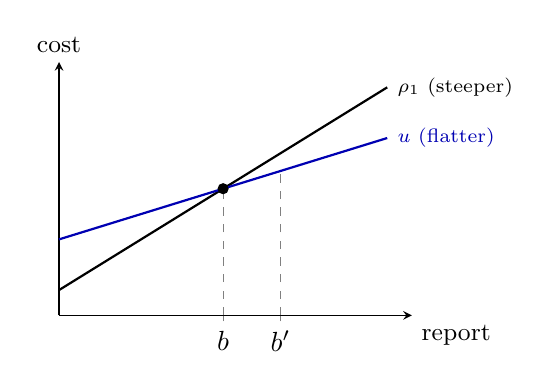
\begin{tikzpicture}
\begin{axis}[width=0.5\textwidth, height=4.8cm, xmin=2, xmax=6.3, ymin=2.5, ymax=7.5,
  axis lines=left, xtick={4,4.7}, xticklabels={$b$,$b'$}, ytick=\empty,
  xlabel={report}, ylabel={cost}, clip=false,
  every axis x label/.style={at={(ticklabel* cs:1)}, anchor=north west, font=\small},
  every axis y label/.style={at={(ticklabel* cs:1)}, anchor=south, font=\small}]
\addplot[domain=2:6, thick, black] {1+1.0*x} node[pos=1, right, font=\scriptsize] {$\rho_1$ (steeper)};
\addplot[domain=2:6, thick, blue!70!black] {3+0.5*x} node[pos=1, right, font=\scriptsize] {$u$ (flatter)};
\draw[dashed, gray] (axis cs:4,2.5) -- (axis cs:4,5);
\draw[dashed, gray] (axis cs:4.7,2.5) -- (axis cs:4.7,5.35);
\addplot[only marks, mark=*, mark size=1.8pt] coordinates {(4,5)};
\end{axis}
\end{tikzpicture}
\caption{Tie-breaking in Step~3 of \cref{lem:substitute}. Two routes with the
same bundle cost the same at $b$. Just to the right of $b$ the flatter one (the
one with less working time) is strictly cheaper; just to the left, the steeper
one. This is why ties cannot block membership in the frontier.}
\label{fig:tiebreak}
\end{figure}

\begin{proof}[Proof of Theorem~\ref{thm:frontier}(a)]
Fix an instance, a profile $b\in\Theta^N$ and an optimal allocation $\rho$ for
the full pools. For every driver $j$ whose route $\rho_j$ is deleted
($\rho_j\notin\Ks_j\cup\{\idle_j\}$), \cref{lem:substitute} gives a kept route
$u_j\in\Ks_j\cup\{\idle_j\}$ with $S_{u_j}\subseteq S_{\rho_j}$ and
$c_{u_j}(b_j)+q(S_{\rho_j}\setminus S_{u_j})\le c_{\rho_j}(b_j)$. Give $u_j$ to
driver $j$ and send $S_{\rho_j}\setminus S_{u_j}$ to FD. Bundles only shrink, so
they stay disjoint; every order is still served exactly once; and no other
driver is affected, so all replacements can be made at the same time. The new
allocation uses only kept routes and costs at most $V(R;b)$. Hence
$V(R^{\Pi^\star};b)\le V(R;b)$; the reverse inequality holds because the pruned
pools are smaller. Removing a driver $k$ gives another instance in which every
remaining driver has the same local view, so the same argument applies to
$V_{-k}$.
\end{proof}

\begin{corollary}[VCG outcomes are preserved]\label{cor:vcg}
Let $\Ks=\bigcup_{i\in N}\Ks_i$ and $b\in\Theta^N$.
\begin{enumerate}[label=(\roman*), itemsep=1pt]
\item Running Algorithms~B and~C on the pruned pools is VCG on a range fixed
before bidding, hence truthful and individually rational (\cref{lem:dsic}).
\item Suppose the full-pool mechanism breaks ties among optimal allocations
first by using as few routes outside $\Ks$ as possible, and then by the same
report-independent rule as the pruned mechanism. Then both select the same
allocation, and every payment \eqref{eq:payment} coincides.
\item If the full problem has a unique optimal allocation at $b$, that
allocation uses only routes of $\Ks$, and (ii) holds under any tie-breaking rule.
\end{enumerate}
\end{corollary}

\begin{proof}
(i) is \cref{lem:dsic}. (ii) The proof of Theorem~1(a) turns every optimal
allocation into one of no larger cost that uses only routes of $\Ks$. So the
optimal allocations that use no route outside $\Ks$ are exactly the optimal
allocations of the pruned problem, which has the same optimal value; the
remaining tie-breaking criteria are the same in both mechanisms. $V$ and every
$V_{-k}$ coincide by Theorem~1(a), so \eqref{eq:payment} coincides. The first
tie-breaking criterion reads no report, so \cref{lem:dsic} also applies to the
full-pool mechanism. (iii) If the unique optimum used a route outside $\Ks$,
the replacement above would produce a different allocation of no larger cost.
\end{proof}

\begin{lemma}[Margin against all other routes]\label{lem:margin}
Let $R_i$ satisfy \cref{ass:down,ass:nofree}, $\thl<\thu$, and $r\in\Ks_i$
with $S:=S_r$. There are $b^*\in\Theta$ and $\gamma>0$ such that
\begin{equation}\label{eq:margin}
c_{r'}(b^*)+q(S\setminus S_{r'})\;\ge\;c_r(b^*)+\gamma
\qquad\text{for every } r'\in R_i\cup\{\idle_i\},\ r'\ne r .
\end{equation}
\end{lemma}

In words: at report $b^*$, replacing $r$ by any other route of driver $i$ ---
whatever orders that route serves --- and sending the orders of $S$ that it
misses to FD costs at least $\gamma$ more. Orders outside $S$ that $r'$ happens
to serve are not counted on the left; they are dealt with in the proof of
Theorem~1(b).

\begin{proof}
\emph{Step 1: an interval of positive margin.} Since $r\in\Ks_i$,
$\mu_r(\bar b)>0$ for some $\bar b\in\Theta$. The margin is continuous
(\cref{lem:lines}), so $\mu_r>0$ on a whole interval $J\subseteq\Theta$ of
positive length around $\bar b$; if $\bar b$ is an end point of $\Theta$, $J$
lies on the inner side, which is possible because $\thl<\thu$.

\emph{Step 2: three cases for $r'$ (\cref{fig:venn}).} Let $b\in J$.

\noindent\emph{(i) $S_{r'}\subseteq S$.} Then $r'$ is a substitute of $r$, so
the left-hand side of \eqref{eq:margin} is at least $E_r(b)=c_r(b)+\mu_r(b)$.

\noindent\emph{(ii) $S_{r'}$ overlaps $S$ partially}, i.e.\
$T:=S\cap S_{r'}\ne S$ and $S_{r'}\not\subseteq S$. By \cref{ass:down} applied
to $r'$ and $T$, there is a route $\hat r$ with $S_{\hat r}=T$ and
$c_{\hat r}(b)\le c_{r'}(b)$. As $T\ne S$, $\hat r$ is a substitute of $r$.
Since $S\setminus S_{r'}=S\setminus T$,
\[
c_{r'}(b)+q(S\setminus S_{r'})\;\ge\;c_{\hat r}(b)+q(S\setminus T)\;\ge\;E_r(b)=c_r(b)+\mu_r(b).
\]

\noindent\emph{(iii) $S\subsetneq S_{r'}$.} Then $q(S\setminus S_{r'})=0$. By
\cref{ass:down} with $T=S$ there is $\hat r$ with $S_{\hat r}=S$ and
$c_{\hat r}(b)\le c_{r'}(b)$. If $\hat r=r$, then $c_{r'}(b)\ge c_r(b)$. If
$\hat r\ne r$, then $\hat r$ is a substitute of $r$ with the same bundle, so
$c_{\hat r}(b)\ge E_r(b)>c_r(b)$. In both cases the line
$h_{r'}(b):=c_{r'}(b)-c_r(b)$ is nonnegative on $J$. By \cref{ass:nofree},
$\pair(r')\ne\pair(r)$, so $h_{r'}$ is not identically zero, and by
\cref{lem:lines}(iii) it is strictly positive on $J$ except at, at most, one
point.

\emph{Step 3: choice of $b^*$ and $\gamma$.} Pick $b^*\in J$ different from the
finitely many exceptional points of case (iii); this is possible because $J$
has positive length. Put
$\gamma=\min\bigl\{\mu_r(b^*),\ \min_{r'\text{ in case (iii)}}h_{r'}(b^*)\bigr\}>0$.
Cases (i) and (ii) give \eqref{eq:margin} because $\mu_r(b^*)\ge\gamma$, and case
(iii) because $h_{r'}(b^*)\ge\gamma$.
\end{proof}

\begin{figure}[!htbp]
\centering
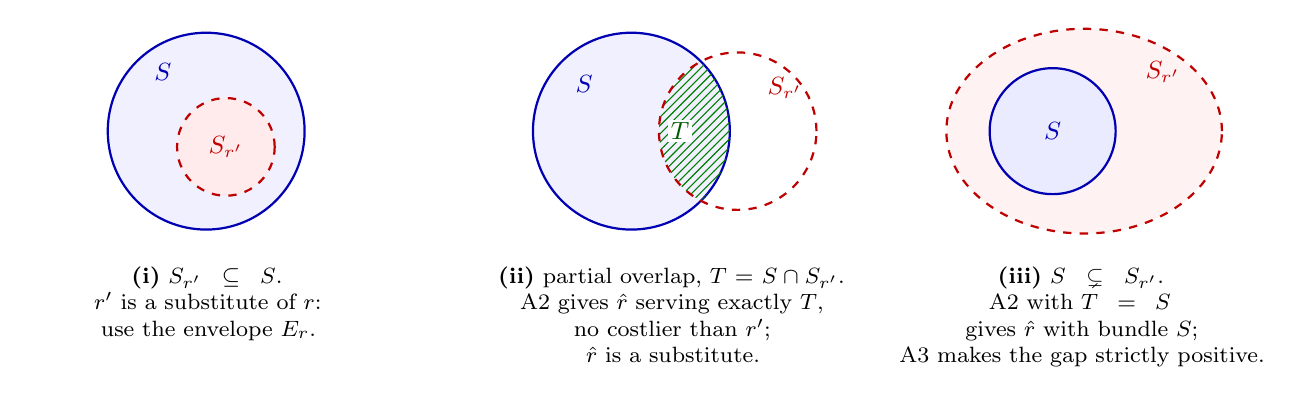
\begin{tikzpicture}[font=\small]
% (i) subset
\begin{scope}
\draw[thick, blue!70!black, fill=blue!6] (0,0) circle (1.25);
\draw[thick, red!75!black, dashed, fill=red!8] (0.25,-0.2) circle (0.62);
\node[blue!70!black] at (-0.55,0.75) {$S$};
\node[red!75!black] at (0.25,-0.2) {$S_{r'}$};
\node[anchor=north, align=center, text width=4.3cm, font=\footnotesize] at (0,-1.6)
  {\textbf{(i)} $S_{r'}\subseteq S$.\\ $r'$ is a substitute of $r$:\\ use the envelope $E_r$.};
\end{scope}
% (ii) partial overlap
\begin{scope}[xshift=5.4cm]
\draw[thick, blue!70!black, fill=blue!6] (0,0) circle (1.25);
\begin{scope}
\clip (0,0) circle (1.25);
\fill[pattern=north east lines, pattern color=green!50!black] (1.35,0) circle (1.0);
\end{scope}
\draw[thick, red!75!black, dashed] (1.35,0) circle (1.0);
\node[blue!70!black] at (-0.6,0.6) {$S$};
\node[red!75!black] at (1.95,0.55) {$S_{r'}$};
\node[green!35!black, fill=white, inner sep=1pt] at (0.62,0) {$T$};
\node[anchor=north, align=center, text width=4.6cm, font=\footnotesize] at (0.5,-1.6)
  {\textbf{(ii)} partial overlap, $T=S\cap S_{r'}$.\\ A2 gives $\hat r$ serving exactly $T$,\\ no costlier than $r'$; $\hat r$ is a substitute.};
\end{scope}
% (iii) superset
\begin{scope}[xshift=11.0cm]
\draw[thick, red!75!black, dashed, fill=red!5] (0.15,0) ellipse (1.75 and 1.3);
\draw[thick, blue!70!black, fill=blue!8] (-0.25,0) circle (0.8);
\node[blue!70!black] at (-0.25,0) {$S$};
\node[red!75!black] at (1.15,0.75) {$S_{r'}$};
\node[anchor=north, align=center, text width=4.6cm, font=\footnotesize] at (0.1,-1.6)
  {\textbf{(iii)} $S\subsetneq S_{r'}$.\\ A2 with $T=S$ gives $\hat r$ with bundle $S$;\\ A3 makes the gap strictly positive.};
\end{scope}
\end{tikzpicture}
\caption{The three ways another route $r'$ of the same driver can relate to the
bundle $S=S_r$ (proof of \cref{lem:margin}). In (ii), downward closure
replaces $r'$ by a route $\hat r$ that serves only the common orders $T$ and is
no more expensive; $\hat r$ is then a substitute of $r$, so the envelope
applies.}
\label{fig:venn}
\end{figure}

\begin{proof}[Proof of Theorem~\ref{thm:frontier}(b)]
Let $b^*$ and $\gamma$ be as in \cref{lem:margin} and fix
$0<\varepsilon\le\gamma/(2B)$.

\emph{Construction (\cref{fig:helpers}).} The instance consists of driver $i$
with report $b^*$ and, for every order $x\notin S$, a \emph{helper} driver $j_x$
whose pool is a single route serving only $\{x\}$ with $K=\varepsilon$ and
$W=0$ (so its report does not matter). The data $O,q,B,\Theta,R_i$ are
unchanged, so driver $i$ has local view $L_i$.

\emph{Evaluation.} Fix the route $r'\in R_i\cup\{\idle_i\}$ that driver $i$
receives, and complete the allocation as cheaply as possible:
\begin{itemize}[leftmargin=1.4em, itemsep=1pt]
\item orders of $S_{r'}$ are served by $i$;
\item orders of $S\setminus S_{r'}$ can only go to FD, since no helper serves
them;
\item every order $x\notin S\cup S_{r'}$ is served by its helper or by FD, at
cost $e_x:=\min\{\varepsilon,q_x\}\le\varepsilon$;
\item for orders $x\in S_{r'}\setminus S$ the helper stays idle.
\end{itemize}
The cheapest allocation in which $i$ receives $r'$ therefore costs
\[
F(r')=c_{r'}(b^*)+q(S\setminus S_{r'})+\sum_{x\notin S\cup S_{r'}}e_x,
\qquad\text{in particular}\qquad
F(r)=c_r(b^*)+\sum_{x\notin S}e_x .
\]
Subtracting, and using \eqref{eq:margin} and $|S_{r'}\setminus S|\le B$,
\[
F(r')-F(r)=\underbrace{c_{r'}(b^*)+q(S\setminus S_{r'})-c_r(b^*)}_{\ge\gamma}
-\underbrace{\sum_{x\in S_{r'}\setminus S}e_x}_{\le B\varepsilon\le\gamma/2}
\;\ge\;\frac{\gamma}{2}\qquad\text{for every }r'\ne r.
\]
Hence every optimal allocation gives $r$ to driver $i$, and
$V(R\setminus\{r\};b)=\min_{r'\ne r}F(r')\ge F(r)+\gamma/2=V(R;b)+\gamma/2$.
\end{proof}

The helpers make every order outside $S$ almost free. A route $r'$ that serves
such orders therefore gains almost nothing from them (at most $B\varepsilon$),
while by \cref{lem:margin} it loses at least $\gamma$ on the orders of $S$.

\begin{figure}[!htbp]
\centering
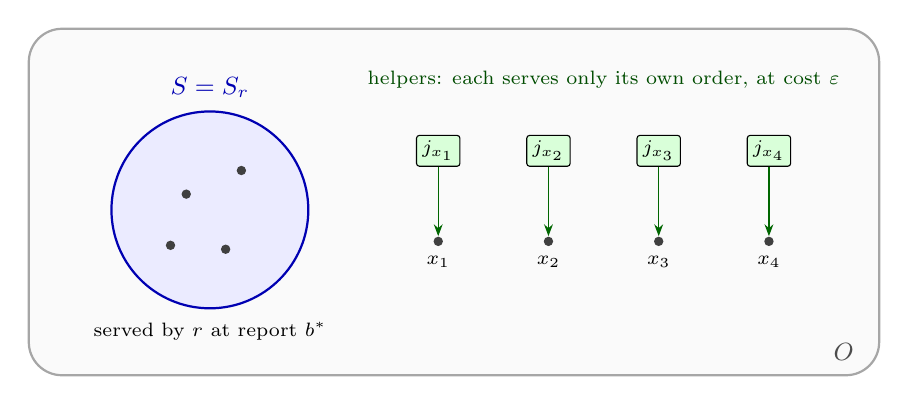
\begin{tikzpicture}[font=\small]
\draw[rounded corners=12pt, thick, gray!70, fill=gray!4] (-1.0,-2.1) rectangle (9.8,2.3);
\node[gray!60!black] at (9.35,-1.8) {$O$};
\draw[thick, blue!70!black, fill=blue!8] (1.3,0) circle (1.25);
\node[blue!70!black, anchor=south] at (1.3,1.3) {$S=S_r$};
\foreach \p in {(1.0,0.2),(1.7,0.5),(1.5,-0.5),(0.8,-0.45)} \node[order] at \p {};
\node[anchor=north, font=\scriptsize] at (1.3,-1.3) {served by $r$ at report $b^*$};
\foreach \x/\lab in {4.2/x_1, 5.6/x_2, 7.0/x_3, 8.4/x_4} {
  \node[order, label={[font=\scriptsize]below:$\lab$}] (o\lab) at (\x,-0.4) {};
  \node[draw, fill=green!15, rounded corners=1pt, font=\scriptsize, inner sep=2pt] (h\lab) at (\x,0.75) {$j_{\lab}$};
  \draw[-{Stealth[length=1.5mm]}, green!40!black] (h\lab) -- (o\lab);
}
\node[align=center, font=\scriptsize, green!30!black] at (6.3,1.65) {helpers: each serves only its own order, at cost $\varepsilon$};
\end{tikzpicture}
\caption{The instance in the proof of Theorem~1(b). Orders outside $S$ become
almost free (cost $\varepsilon$), orders inside $S$ can only be served by
driver $i$ or by FD. Driver $i$'s own data are unchanged, so no local rule can
distinguish this instance from the original one.}
\label{fig:helpers}
\end{figure}

\begin{proof}[Proof of Theorem~\ref{thm:frontier}(c)]
Suppose a local rule $\Pi$ deletes some $r\in\Ks_i$ from a local view $L_i$
that satisfies \cref{ass:down,ass:nofree}. In the instance of part (b), driver
$i$ has local view $L_i$, so $\Pi$ deletes $r$ there as well (and possibly
other routes). Every allocation of the pruned pools is an allocation of
$R\setminus\{r\}$, hence $V(R^\Pi;b)\ge V(R\setminus\{r\};b)>V(R;b)$ and $\Pi$ is
not safe. So every safe local rule deletes only routes outside $\Ks_i$;
$\Pi^\star$ deletes all of them and is safe by part (a).
\end{proof}

% ---------------------------------------------------------------------
\subsection{Theorem 2: the price of locality}
\label{sec:thm2}
% ---------------------------------------------------------------------

Theorem~1 says what a local rule must keep. Theorem~2 shows that this can be a
great deal, and that all of it can be useless.

\begin{theorem}[Price of locality]\label{thm:pol}
Fix $B\ge1$. For every $n\ge B$ there is a Euclidean instance $I_n$ with $n$
orders, one gigworker $g$ and $n$ occasional drivers such that
\begin{enumerate}[label=(\roman*), itemsep=1pt]
\item $R_g$ contains exactly one route for each bundle of at most $B$ orders,
all of them in $\Ks_g$; hence every safe local rule keeps
$\sum_{k=1}^{B}\binom nk=\Theta(n^B)$ routes of $g$;
\item for every report profile in $\Theta^{n+1}$, no optimal allocation assigns
a route to $g$.
\end{enumerate}
\end{theorem}

\paragraph{Construction (\cref{fig:pol}).} All $n$ orders are picked up at the
same point $P$ and delivered at the same point $D$, with $d(P,D)=\ell$, release
time $0$, non-binding deadlines, service time $s$ (minutes) per stop and a
common FD price $q_0$. The gigworker starts at $A$, with $d(A,P)=a$, at time
$0$, with capacity at least $B$ and distance coefficient $\kappa>0$. Each
occasional driver $\omega_1,\dots,\omega_n$ travels from $P$ to $D$, departs at
time $0$ and has detour budget $2s$. Let $T_0=\tau(A,P)+\tau(P,D)$. The
parameters satisfy
\begin{align}
&q_0>2s\,\thu/60, \tag{C1}\label{eq:C1}\\
&\kappa(a+\ell)+\thl\,(T_0+2s)/60<q_0, \tag{C2}\label{eq:C2}\\
&\kappa(a+\ell)>B\,(\thu-\thl)\,2s/60. \tag{C3}\label{eq:C3}
\end{align}
For example, $B=3$, $s=2$~min, $\Theta=[18,25]$, $\kappa=0.5$, $a=2$~km,
$\ell=6$~km, speed $20$~km/h and $q_0=20$ give $T_0=24$~min and
(C1)~$20>1.67$, (C2)~$12.4<20$, (C3)~$4>1.4$. (Condition (C3) depends on $B$;
with these numbers it holds for $B\le8$.)

\begin{figure}[!htbp]
\centering
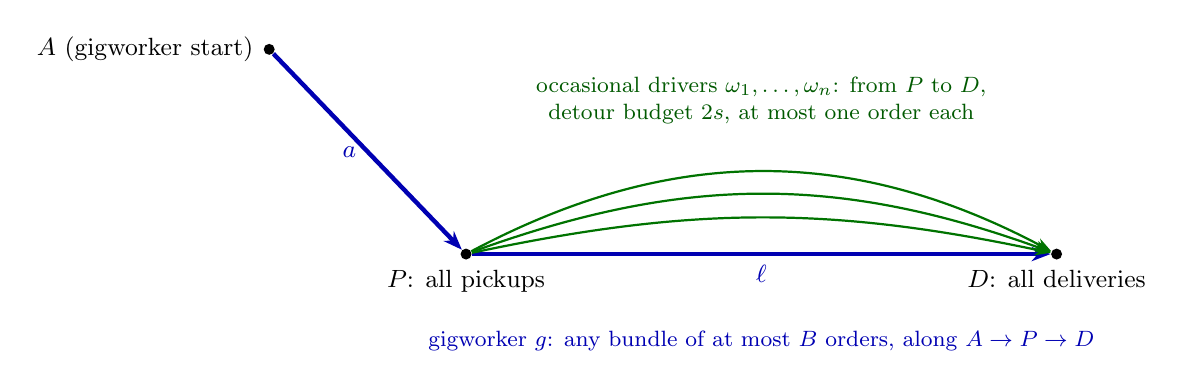
\begin{tikzpicture}[font=\small, x=1cm, y=1cm]
\node[stop, label=left:{$A$ (gigworker start)}] (A) at (0,2.6) {};
\node[stop, label=below:{$P$: all pickups}] (P) at (2.5,0) {};
\node[stop, label=below:{$D$: all deliveries}] (D) at (10,0) {};
\draw[-{Stealth[length=2.4mm]}, ultra thick, blue!70!black] (A) -- node[left, pos=0.5] {$a$} (P);
\draw[-{Stealth[length=2.4mm]}, ultra thick, blue!70!black] (P) -- node[below, pos=0.5] {$\ell$} (D);
\draw[-{Stealth[length=2mm]}, thick, green!45!black] (P) to[bend left=12] (D);
\draw[-{Stealth[length=2mm]}, thick, green!45!black] (P) to[bend left=20] (D);
\draw[-{Stealth[length=2mm]}, thick, green!45!black] (P) to[bend left=28] (D);
\node[green!35!black, align=center, font=\footnotesize] at (6.25,1.95) {occasional drivers $\omega_1,\dots,\omega_n$: from $P$ to $D$,\\ detour budget $2s$, at most one order each};
\node[blue!70!black, align=center, font=\footnotesize] at (6.25,-1.1) {gigworker $g$: any bundle of at most $B$ orders, along $A\to P\to D$};
\end{tikzpicture}
\caption{The instance of Theorem~2. The gigworker can serve every bundle of up
to $B$ orders along the same path, so her pool has one route per bundle, and
none of these routes can be removed by a local rule. Yet the occasional
drivers serve every order more cheaply, one each, so the gigworker never wins.}
\label{fig:pol}
\end{figure}

\begin{proof}
\emph{Step 1: the gigworker's pool.} For a bundle $S$ with $|S|=k\le B$, every
sequence that performs all pickups at $P$ before all deliveries at $D$ has
length $a+\ell$ and completion time $T_0+2sk$ (no waiting). Every other sequence
returns from $D$ to $P$ at least once, so it is at least $2\ell$ longer and
finishes later; it is Pareto-dominated. Hence $R_g=\{r_S\}$ with
$K_{r_S}=\kappa(a+\ell)$ and $W_{r_S}=(T_0+2sk)/60$, one route per bundle.
\Cref{ass:nodup,ass:down} hold by \cref{lem:downward}, and \cref{ass:nofree}
holds because $W_{r_S}$ increases strictly with $|S|$.

\emph{Step 2: every route is in the frontier.} Take $b=\thl$ and a bundle $S$
with $|S|=k$. The substitutes of $r_S$ are $r_{S'}$ for
$\emptyset\ne S'\subsetneq S$ and $\idle_g$. For the former,
\[
c_{r_{S'}}(b)+q_0(k-|S'|)-c_{r_S}(b)=(k-|S'|)\bigl(q_0-2sb/60\bigr)>0
\]
by (C1), since the two routes have the same $K$ and differ by $2s(k-|S'|)$
minutes of working time. For the idle option,
\[
q_0k-c_{r_S}(b)=\bigl(q_0-c_{r_{\{x\}}}(b)\bigr)+(k-1)\bigl(q_0-2sb/60\bigr)>0
\]
by (C2) and (C1), where $r_{\{x\}}$ is any single-order route. Hence
$\mu_{r_S}(\thl)>0$, so $r_S\in\Ks_g$, and by Theorem~1(c) every safe local
rule keeps it. This proves (i).

\emph{Step 3: the gigworker never wins.} Each $\omega_j$ can serve any single
order with zero extra distance and extra time $2s$ (the two service stops), and
cannot serve two orders, which would need an extra time of at least $4s$. Take
an allocation in which $g$ serves $r_S$ with $|S|=k$. The $n-k$ orders outside
$S$ occupy at most $n-k$ occasional drivers, so at least $k$ of them are idle.
Give the orders of $S$ to $k$ idle occasional drivers and make $g$ idle. The
reported cost changes by at most
\[
-c_{r_S}(b_g)+k\,\thu\,\frac{2s}{60}
\;\le\;-\kappa(a+\ell)-\thl\,\frac{T_0+2sk}{60}+k\,\thu\,\frac{2s}{60}
\;\le\;-\kappa(a+\ell)+B(\thu-\thl)\frac{2s}{60}\;<\;0
\]
by (C3). So no allocation that uses a route of $g$ is optimal. This proves (ii).
\end{proof}

The theorem makes the asymmetry between the driver classes precise: nothing
bounds the pool that no local rule can shrink except feasibility. A tight
detour budget restricts feasibility; time windows alone do not.
\Cref{rem:polod} shows that an occasional driver with a generous detour budget
is exposed in exactly the same way.

% ---------------------------------------------------------------------
\subsection{Theorem 3: an FD-completion label rule}
\label{sec:label}
% ---------------------------------------------------------------------

The frontier is computed after Algorithm~A has enumerated every route. This
subsection moves part of the test inside the enumeration. When a partial route
(a label) has picked up a set $T$ of orders, we bound from below how much any
completion of it would save by dropping $T$ and sending $T$ to FD. If that
saving is at least the FD price $q(T)$, the label and all its extensions are
discarded. By Theorem~1(c) no rule of this kind can shrink the frontier; what
is at stake is only the running time of Algorithm~A.

\paragraph{Labels and shortcuts.} Fix a driver with start $v_0$, departure
$t_0$ and coefficient $\kappa$. A label is identified with its stop sequence
$L=(v_1,\dots,v_m)$, with service starts and ready times \eqref{eq:recursion};
$D$ is its length and $r=r_m$ its ready time at its last stop $v_m$. $P(L)$ is
the set of orders picked up in $L$.

\begin{definition}[Shortcut quantities]\label{def:shortcut}
Let $\emptyset\ne T\subseteq P(L)$, and let $L\setminus T$ be the subsequence
of $L$ without the stops of the orders of $T$, with last point $v'$, ready time
$r'$ there, and length $D'$ ($v'=v_0$, $r'=t_0$, $D'=0$ if $L\setminus T$ is
empty). Let $\mathcal F(L)$ be the set of stops with an opening time that a
feasible continuation of $L$ may still visit: the pickups $p_j$ of orders
$j\notin P(L)$ with $r+\tau(v_m,p_j)\le l_{p_j}$ (none if $|P(L)|=B$), and, if
deliveries have opening times, the deliveries of orders on board at the end of
$L$ and of orders whose pickups are in $\mathcal F(L)$. Define
\begin{align*}
\Delta D(L,T)&=D-D'-d(v',v_m) &&\text{(distance spent on $T$)},\\
\delta(L,T)&=r-r'-\tau(v',v_m) &&\text{(time spent on $T$)},\\
A(L,T)&=\max\Bigl\{0,\ \max_{w\in\mathcal F(L)}\bigl(e_w-r'-\tau(v',w)\bigr)\Bigr\}
&&\text{(time that later waiting can absorb)},\\
\beta(L,T)&=\kappa\,\Delta D(L,T)+\thl\,\frac{\max\{0,\ \delta(L,T)-A(L,T)\}}{60}
&&\text{(guaranteed saving)}.
\end{align*}
The \emph{FD-completion label rule} discards $L$ and all its extensions if
$\beta(L,T)\ge q(T)$ for some $\emptyset\ne T\subseteq P(L)$.
\end{definition}

The two corrections are what makes the rule safe (\cref{fig:junction}). The
\emph{junction terms} $d(v',v_m)$ and $\tau(v',v_m)$ account for the fact that
the continuation of $L$ starts at $v_m$, whereas the shortcut ends at $v'$: the
shortcut still has to get to wherever the route goes next. The
\emph{absorption term} $A$ accounts for waiting: a route that is ahead in time
may simply wait longer at a later stop that has not opened yet, so part of its
time saving can disappear (\cref{fig:absorb}).

\begin{figure}[!htbp]
\centering
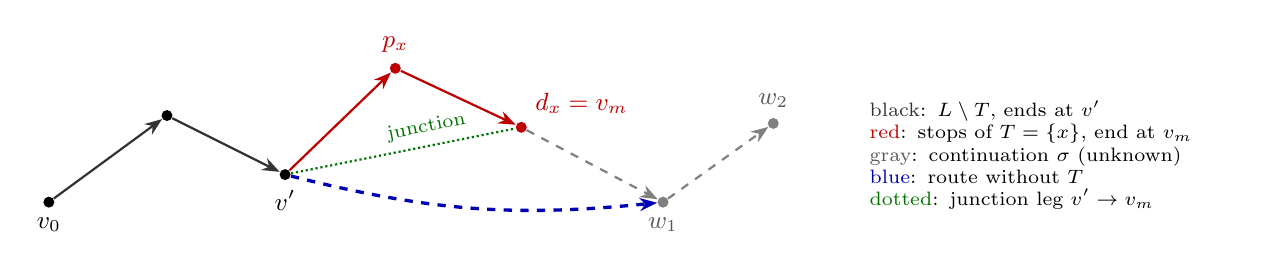
\begin{tikzpicture}[font=\small, x=1cm, y=1cm]
\node[stop, label=below:{$v_0$}] (v0) at (0,0) {};
\node[stop] (u1) at (1.5,1.1) {};
\node[stop, label=below:{$v'$}] (vp) at (3.0,0.35) {};
\node[stop, red!75!black, label={[red!75!black]above:{$p_x$}}] (px) at (4.4,1.7) {};
\node[stop, red!75!black, label={[red!75!black]above right:{$d_x=v_m$}}] (dx) at (6.0,0.95) {};
\node[stop, gray, label={[gray!70!black]below:{$w_1$}}] (w1) at (7.8,0.0) {};
\node[stop, gray, label={[gray!70!black]above:{$w_2$}}] (w2) at (9.2,1.0) {};
\draw[arr, black!80] (v0) -- (u1);
\draw[arr, black!80] (u1) -- (vp);
\draw[arr, red!75!black] (vp) -- (px);
\draw[arr, red!75!black] (px) -- (dx);
\draw[arr, gray, dashed] (dx) -- (w1);
\draw[arr, gray, dashed] (w1) -- (w2);
\draw[arr, blue!70!black, very thick, dashed] (vp) to[bend right=10] (w1);
\draw[densely dotted, thick, green!45!black] (vp) -- node[above, sloped, font=\scriptsize, pos=0.62] {junction} (dx);
\node[align=left, anchor=west, text width=4.6cm, font=\scriptsize] at (10.3,0.6)
{\textcolor{black!80}{black}: $L\setminus T$, ends at $v'$\\
\textcolor{red!75!black}{red}: stops of $T=\{x\}$, end at $v_m$\\
\textcolor{gray!70!black}{gray}: continuation $\sigma$ (unknown)\\
\textcolor{blue!70!black}{blue}: route without $T$\\
\textcolor{green!45!black}{dotted}: junction leg $v'\to v_m$};
\end{tikzpicture}
\caption{The shortcut of a label. Dropping order $x$ replaces the red stretch
and the first gray leg by the blue leg. The saving in distance is at least
$D-D'-d(v',v_m)$, by the triangle inequality $d(v',w_1)\le d(v',v_m)+d(v_m,w_1)$;
this holds whatever the continuation is. Without the junction term the bound
would credit the whole red stretch even when it lies on the way to $w_1$.}
\label{fig:junction}
\end{figure}

\begin{theorem}[The label rule preserves the frontier]\label{thm:preserve}
Let $R_i$ be the pool of Algorithm~A without Layer~3, and $R'_i$ the pool
obtained when Algorithm~A in addition discards some or all labels that satisfy
the rule, together with their extensions. Under the standing assumptions and
$\thl<\thu$,
\[
\Ks_i(R'_i)=\Ks_i(R_i),
\]
with routes identified by their bundle and pair. Consequently, applying the
rule and then $\Pi^\star$ produces the same pool as $\Pi^\star$ alone, and
Theorem~1 and \cref{cor:vcg} apply unchanged.
\end{theorem}

The proof needs two ingredients: \cref{lem:absorb}, which quantifies how much
of a time lead survives waiting, and \cref{prop:labelbound}, which shows that
$\beta$ is a valid lower bound on the saving for every completion.

\begin{lemma}[Absorption of a time lead]\label{lem:absorb}
Two paths visit the same stops $w_1,\dots,w_k$ in this order. Path~1 leaves
point $x$ at time $\eta$, path~2 leaves point $x'$ at time $\eta'$. Let
$T_1=\eta'+\tau(x',w_1)$ and $T_{j+1}=T_j+s_{w_j}+\tau(w_j,w_{j+1})$ be the
arrival times of path~2 if it never waited. If path~1 reaches $w_1$ at least
$\delta$ later than $T_1$, i.e.\ $\eta+\tau(x,w_1)\ge T_1+\delta$, then for every
$j$ the service starts satisfy
\[
a^{(1)}_j-a^{(2)}_j\;\ge\;\delta-\max_{l\le j}\,\bigl(e_{w_l}-T_l\bigr)^+ .
\]
\end{lemma}

In words: path~2 has a lead of $\delta$. Waiting at a stop $w_l$ can eat at
most $(e_{w_l}-T_l)^+$ of that lead, namely the time by which path~2 would have
arrived before the stop opens.

\begin{proof}
Write $\mathrm{dur}(l\to j)=\sum_{h=l}^{j-1}(s_{w_h}+\tau(w_h,w_{h+1}))$ for the
no-wait travel and service time from $w_l$ to $w_j$. Unrolling
\eqref{eq:recursion} shows that a path arriving at $w_1$ at time $U_1$ starts
service at $w_j$ at
\[
a_j=\max\bigl\{U_1+\mathrm{dur}(1\to j),\ M_j\bigr\},\qquad
M_j=\max_{l\le j}\bigl\{e_{w_l}+\mathrm{dur}(l\to j)\bigr\}:
\]
either the driver never waited, or the start is forced by the last opening time
at which she waited. $M_j$ is the same for both paths. For path~2,
$U_1=T_1$ and $T_1+\mathrm{dur}(1\to j)=T_j$, so $a^{(2)}_j=\max\{T_j,M_j\}$; for
path~1, $U_1\ge T_1+\delta$, so $a^{(1)}_j\ge\max\{T_j+\delta,M_j\}$. If
$M_j\le T_j$ the difference is at least $\delta$; if $T_j<M_j\le T_j+\delta$ it
is at least $T_j+\delta-M_j$; otherwise it is at least $0$. In every case it is
at least $\delta-(M_j-T_j)^+$, and $M_j-T_j=\max_{l\le j}(e_{w_l}-T_l)$ because
$T_j=T_l+\mathrm{dur}(l\to j)$.
\end{proof}

\begin{figure}[!htbp]
\centering
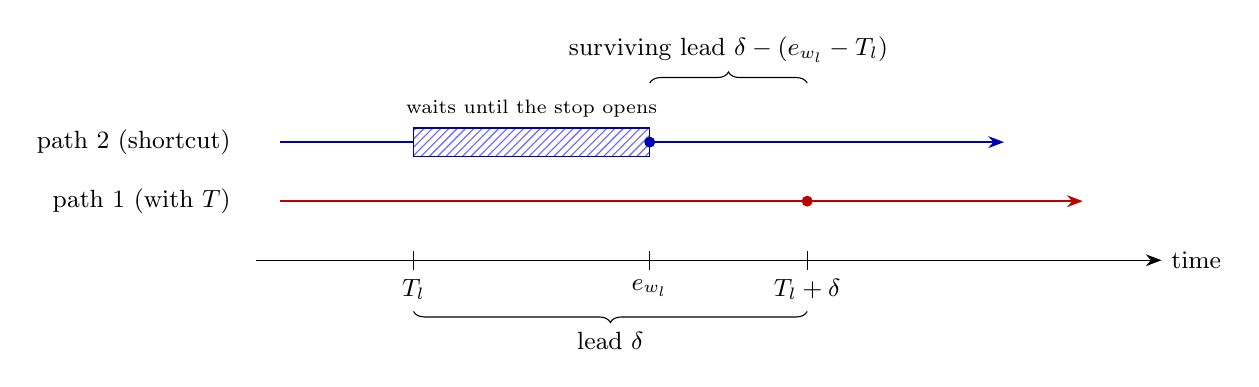
\begin{tikzpicture}[font=\small, x=1cm, y=1cm]
\draw[-{Stealth[length=2mm]}] (0,0) -- (11.5,0) node[right] {time};
\foreach \x/\lab in {2/T_l, 5/e_{w_l}, 7/T_l+\delta} {
  \draw (\x,0.12) -- (\x,-0.12) node[below] {$\lab$};
}
% path 2
\node[anchor=east] at (-0.2,1.5) {path 2 (shortcut)};
\draw[thick, blue!70!black] (0.3,1.5) -- (2,1.5);
\fill[pattern=north east lines, pattern color=blue!60] (2,1.32) rectangle (5,1.68);
\draw[blue!70!black] (2,1.32) rectangle (5,1.68);
\node[font=\scriptsize] at (3.5,1.92) {waits until the stop opens};
\draw[thick, blue!70!black, -{Stealth[length=2mm]}] (5,1.5) -- (9.5,1.5);
\node[stop, blue!70!black] at (5,1.5) {};
% path 1
\node[anchor=east] at (-0.2,0.75) {path 1 (with $T$)};
\draw[thick, red!75!black] (0.3,0.75) -- (7,0.75);
\draw[thick, red!75!black, -{Stealth[length=2mm]}] (7,0.75) -- (10.5,0.75);
\node[stop, red!75!black] at (7,0.75) {};
\draw[decorate, decoration={brace, amplitude=4pt, mirror}] (2,-0.65) -- (7,-0.65) node[midway, below=4pt] {lead $\delta$};
\draw[decorate, decoration={brace, amplitude=4pt}] (5,2.25) -- (7,2.25) node[midway, above=4pt] {surviving lead $\delta-(e_{w_l}-T_l)$};
\end{tikzpicture}
\caption{Absorption of a time lead (\cref{lem:absorb}). The route without $T$
(path~2) would reach stop $w_l$ at $T_l$, but the stop opens only at $e_{w_l}$, so
it waits. Of the original lead $\delta$ only $\delta-(e_{w_l}-T_l)$ survives.
The term $A$ in \cref{def:shortcut} bounds the largest such loss over all stops
that a continuation may visit.}
\label{fig:absorb}
\end{figure}

\begin{proposition}[Label bound]\label{prop:labelbound}
Let $L$ be a label, $\emptyset\ne T\subseteq P(L)$, and $\rho$ any feasible
route of the driver that starts with $L$ (possibly $\rho=L$). Let $\rho\setminus T$
be $\rho$ without the stops of the orders of $T$. Then
\[
K_\rho-K_{\rho\setminus T}\ge\kappa\,\Delta D(L,T),\qquad
W_\rho-W_{\rho\setminus T}\ge\frac{\max\{0,\ \delta(L,T)-A(L,T)\}}{60},
\]
and therefore $c_\rho(b)-c_{\rho\setminus T}(b)\ge\beta(L,T)$ for every
$b\ge\thl$. In particular, if the rule fires for $(L,T)$, then
$c_\rho(b)\ge c_{\rho\setminus T}(b)+q(T)$ for every $b\in\Theta$: inside every
completion of $L$, serving $T$ costs at least as much as giving $T$ to FD.
\end{proposition}

\begin{proof}
Write $\rho=L\cdot\sigma$, where $\sigma$ is the continuation, and introduce the
intermediate sequence $\pi=(L\setminus T)\cdot\sigma$ (the stops of $T$ are
removed from $L$ only). Removing from $\pi$ the stops of $T$ that lie in
$\sigma$ (deliveries of orders of $T$ still on board at the end of $L$) gives
$\rho\setminus T$. By \cref{lem:remove}, $K_\pi\ge K_{\rho\setminus T}$ and
$W_\pi\ge W_{\rho\setminus T}$, and also $W_\rho\ge W_{\rho\setminus T}$. So it
suffices to show $K_\rho-K_\pi\ge\kappa\Delta D$ and $W_\rho-W_\pi\ge(\delta-A)/60$.

\emph{Distance.} If $\sigma$ is empty, the difference in length is
$D-D'\ge\Delta D$. Otherwise let $u$ be the first point of $\sigma$ (for an
occasional driver possibly the destination). The two sequences differ only up
to $u$, so the difference in length is
$D+d(v_m,u)-D'-d(v',u)\ge D-D'-d(v',v_m)=\Delta D$, because
$d(v',u)\le d(v',v_m)+d(v_m,u)$ (\cref{fig:junction}). For an occasional driver
the same direct length is subtracted from both.

\emph{Time.} If $\sigma$ is empty, $W_\rho-W_\pi=(r-r')/60\ge\delta/60$.
Otherwise apply \cref{lem:absorb} to the stops $w_1,w_2,\dots$ of $\sigma$, with
path~1 $=\rho$ leaving $v_m$ at $r$ and path~2 $=\pi$ leaving $v'$ at $r'$. Its
hypothesis holds: by the triangle inequality
$\tau(v',w_1)\le\tau(v',v_m)+\tau(v_m,w_1)$, so
$r+\tau(v_m,w_1)\ge r'+\tau(v',w_1)+\delta$. At the last stop, or at the
destination, the times therefore differ by at least
$\delta-\max_l(e_{w_l}-T_l)^+$. It remains to show
$\max_l(e_{w_l}-T_l)^+\le A$. A stop $w_l$ of $\sigma$ with an opening time is
either a pickup of an order not picked up in $L$ --- which requires
$|P(L)|<B$, and feasibility of $\rho$ together with the triangle inequality
gives $r+\tau(v_m,w_l)\le l_{w_l}$ --- or the delivery of an order on board or
picked up later. In all cases $w_l\in\mathcal F(L)$. Since
$T_l\ge r'+\tau(v',w_l)$ (triangle inequality, nonnegative service), we get
$e_{w_l}-T_l\le e_{w_l}-r'-\tau(v',w_l)\le A$.

\emph{Cost.} $c_\rho(b)-c_{\rho\setminus T}(b)=(K_\rho-K_{\rho\setminus T})
+b\,(W_\rho-W_{\rho\setminus T})$, and the second difference is nonnegative, so
for $b\ge\thl$ this is at least
$\kappa\Delta D+\thl\max\{0,\delta-A\}/60=\beta$.
\end{proof}

\begin{proof}[Proof of Theorem~\ref{thm:preserve}]
Let $\mathcal F$ be the set of feasible routes of driver $i$. By
\cref{lem:complete}, $R_i$ contains exactly one route for each Pareto-minimal
pair of each bundle, and every route of $\mathcal F$ satisfies alternative (a)
or (b) of \cref{lem:complete} with respect to $R'_i$. Write $D_R(r)$, $E^R_r$,
$\mu^R_r$ for the substitutes, envelope and margin computed in a pool $R$.

\emph{Step 1: routes hit by the rule are outside the frontier.} Let $\rho\in R_i$
satisfy alternative (b) with respect to $R'_i$: a feasible $\tilde\rho$ with the
same bundle and $\pair(\tilde\rho)\le\pair(\rho)$ passes through a label
discarded with witness $T$. By \cref{prop:labelbound},
$c_{\tilde\rho}(b)\ge c_{\tilde\rho\setminus T}(b)+q(T)$ for all $b\in\Theta$.
The route $\tilde\rho\setminus T$ is feasible (as in the proof of
\cref{lem:downward}), so by \cref{lem:complete} without Layer~3 there is
$\hat\rho\in R_i\cup\{\idle_i\}$ with bundle $S_\rho\setminus T$ and
$c_{\hat\rho}\le c_{\tilde\rho\setminus T}$. As $\hat\rho$ is a substitute of
$\rho$,
\[
E^{R_i}_\rho(b)\le c_{\hat\rho}(b)+q(T)\le c_{\tilde\rho\setminus T}(b)+q(T)\le c_{\tilde\rho}(b)\le c_\rho(b)
\qquad\text{for all }b\in\Theta,
\]
so $\mu^{R_i}_\rho\le0$ on $\Theta$ and $\rho\notin\Ks_i(R_i)$.

\emph{Step 2: every frontier route survives.} Let $r\in\Ks_i(R_i)$. By Step~1,
alternative (b) fails for $r$, so (a) holds: $R'_i$ contains a route with bundle
$S_r$ and pair at most $\pair(r)$. As $r$ is Pareto-minimal, that pair is
$\pair(r)$, so $r\in R'_i$.

\emph{Step 3: frontier routes stay in the frontier.} Let $r\in\Ks_i(R_i)$; then
$r\in R'_i$ by Step~2. A substitute of $r$ in $R'_i$ is either a substitute of
$r$ in $R_i$, or a route $r_2\notin R_i$. In the second case $\pair(r_2)$ is not
Pareto-minimal, so $r_2$ is dominated by some $r_1\in R_i$ with the same bundle;
and $r_1\ne r$, because $r\in R'_i$ would otherwise have removed $r_2$ in
Layer~2. So $r_1$ is a substitute of $r$ in $R_i$ and
$c_{r_2}(b)+q(S_r\setminus S_{r_2})\ge c_{r_1}(b)+q(S_r\setminus S_{r_1})\ge E^{R_i}_r(b)$.
Hence $E^{R'_i}_r\ge E^{R_i}_r$ on $\Theta$, so $\mu^{R'_i}_r\ge\mu^{R_i}_r$ and
$r\in\Ks_i(R'_i)$.

\emph{Step 4: no other route enters the frontier.} Let $r\in R'_i$ with
$r\notin\Ks_i(R_i)$. If $r\in R_i$, \cref{lem:substitute} (in $R_i$) gives for
each $b$ a route $u\in\Ks_i(R_i)\cup\{\idle_i\}$ with $S_u\subseteq S_r$ and
$c_u(b)+q(S_r\setminus S_u)\le c_r(b)$; by Step~2, $u\in R'_i\cup\{\idle_i\}$,
and $u\ne r$. So $\mu^{R'_i}_r\le0$ on $\Theta$. If $r\notin R_i$, then $r$ is
dominated by some $r_1\in R_i$ with the same bundle. The pair of $r_1$ does not
occur in $R'_i$ (otherwise Layer~2 would have removed $r$), so alternative (a)
fails for $r_1$; hence (b) holds and $r_1\notin\Ks_i(R_i)$ by Step~1.
\Cref{lem:substitute} applied to $r_1$ gives $u\in\Ks_i(R_i)\cup\{\idle_i\}
\subseteq R'_i\cup\{\idle_i\}$ with
$c_u(b)+q(S_r\setminus S_u)\le c_{r_1}(b)\le c_r(b)$, and $u\ne r$ because
$r\notin R_i$. In both cases $r\notin\Ks_i(R'_i)$.

Steps 3 and 4 give $\Ks_i(R'_i)=\Ks_i(R_i)$.
\end{proof}

Theorem~3 also covers the interaction with label dominance. A label removed by
Layer~1 in favour of another label is never extended, so if an extension of the
dominating label is later discarded by the rule, routes through the dominated
label are lost although no label on their own path satisfies the rule.
\Cref{lem:complete}(b) says exactly that every such route is weakly dominated
by a route through a discarded label, and Step~1 places it outside the frontier.

% =====================================================================
\FloatBarrier
\section{Remarks, algorithms and computational evidence}
\label{sec:remarks}
% =====================================================================

This section is not needed for the proofs of \cref{sec:main}. It collects
remarks on the scope of the results, the procedures that compute them, and the
evidence from the audits and experiments.

% ---------------------------------------------------------------------
\subsection{What the frontier is not}
% ---------------------------------------------------------------------

\begin{remark}[Three ways to beat the frontier]\label{rem:scope}
The minimality in Theorem~1(c) is relative to local rules
(\cref{def:local}). The frontier can be beaten in three ways, each of which
leaves that class.
(i) \emph{Non-local rules} that also read other drivers' public data remain
bid-independent and keep truthfulness; in the instances of Theorem~2 such a rule
could delete every route of the gigworker. Deciding exactly what a non-local
rule may delete is, however, NP-hard (\cref{prop:nonlocal}).
(ii) \emph{Instance-specific rules}, which only need to be correct on the
instance at hand, can keep far less: on five experimental instances only
0.4--1.5\% of generated routes are optimal for any of 1,000 sampled report
profiles, whereas the frontier keeps 3.2--23.1\% of the pool.
(iii) \emph{Restricting the competitors} to geometrically realisable drivers
weakens the safety requirement; \cref{rem:realisable} bounds the effect.
\end{remark}

\begin{proposition}[Exact non-local pruning is hard]\label{prop:nonlocal}
For $B\ge3$ it is NP-hard to decide, given the pools of all drivers, the prices
$q$ and a route $r$, whether $V(R\setminus\{r\};b)=V(R;b)$ for every
$b\in\Theta^N$, even if every route lies in the local frontier of its driver and
no cost depends on the report.
\end{proposition}

\begin{proof}
Reduction from exact cover by 3-sets \citep{garey1979computers}: a universe $U$
with $|U|=3m$ and a family $\mathcal S$ of 3-subsets of $U$. The orders are
$U\cup\{o^\ast\}$, all with $q_o=1$. For each $F\in\mathcal S$ a driver owns one
route serving $F$ at cost $0$; a driver $h$ owns one route for each single order
of $U\cup\{o^\ast\}$, each at cost $0$; and a driver $i$ owns one route $r$ serving
$\{o^\ast\}$ with $K_r=\tfrac12$, $W_r=0$. Every route is cheaper than the FD
price of its bundle and its driver has no route with a smaller bundle, so every
route lies in its driver's frontier.

If an exact cover exists, the sets cover $U$ and $h$ serves $o^\ast$:
$V(R)=V(R\setminus\{r\})=0$. Otherwise a maximum packing of $\mathcal S$ leaves
$u\ge3$ elements uncovered, and any other packing leaves at least $u+3$. Without
$r$, $h$ serves one of the $u+1$ uncovered orders and the rest go to FD, so the
optimal value is $u$. With $r$, $h$ serves an uncovered element and $r$ serves
$o^\ast$, giving $u-1+\tfrac12=u-\tfrac12<u$. Hence $r$ can be deleted safely if
and only if an exact cover exists.
\end{proof}

\begin{remark}[Realisable competitors]\label{rem:realisable}
The helpers $j_x$ in the proof of Theorem~1(b) are abstract. They can be
replaced by genuine occasional drivers whose origin and destination are the
pickup and delivery of $x$ and whose detour budget equals the total service
time $s_x$ at the two stops. Under a general-position condition (no other order
has its pickup and delivery, in this order, on the segment from $p_x$ to $d_x$)
such a driver can serve $x$ and nothing else, with zero extra distance and
working time $s_x/60$, so at report $\thl$ its cost is
$\lambda_x=\thl s_x/60$ (1.20 in the audit setting with $s_x=4$~min; 3.00 with
the five-minute service of the experiments). Repeating the proof of
Theorem~1(b) with $\min\{\lambda_x,q_x\}$ in place of $\min\{\varepsilon,q_x\}$
shows that every frontier route whose margin $\gamma$ in \cref{lem:margin}
exceeds $\sum_{x\in S_{r'}\setminus S}\min\{\lambda_x,q_x\}$ for all $r'$ (for
instance $\gamma>B\thl\max_x s_x/60$) stays indispensable against such
competitors. In a synthetic audit, 556 of 563 frontier routes (98.8\%) did.
Whether a safe local rule could exploit this credit in general is open: a
gigworker route with waiting slack can absorb an extra order at zero extra
working time.
% VERIFY: whether the margin condition, rather than a full instance solve,
% was the criterion behind 556/563 in the audit.
\end{remark}

% ---------------------------------------------------------------------
\subsection{Loose feasibility, not the driver class}
% ---------------------------------------------------------------------

\begin{remark}[Theorem 2 for occasional drivers]\label{rem:polod}
The proof of Theorem~2 uses only that every bundle is feasible, that one
sequence per bundle is Pareto-minimal, and that $K$ is constant and $W$ affine
in $|S|$. It therefore applies to an occasional driver with origin $A$,
destination $D$ and detour budget at least $\tau(A,P)+\tau(P,D)-\tau(A,D)+2sB$
in place of $g$. Her routes have $K_{r_S}=\kappa(a+\ell-d(A,D))$ and
$W_{r_S}=(T_0-\tau(A,D)+2s|S|)/60$, and the proof holds with $a+\ell$ and $T_0$
replaced by $a+\ell-d(A,D)$ and $T_0-\tau(A,D)\ge0$. With $P=(0,0)$, $D=(6,0)$,
$A=(0,4)$ (km), $\kappa=1$, and $B$, $s$, $\Theta$, speed and $q_0$ as in the
example, (C1)--(C3) hold (the left-hand side of (C3) is $2.79$ against $1.40$,
and (C2) reads $6.50<20$), and a detour budget of $20.4$~min suffices, below
the $30$~min used in the experiments. What Theorem~2 separates is loose from
tight feasibility, not one driver class from the other.
\end{remark}

\begin{remark}[Choice of the evaluation point]
The proof of Theorem~2 evaluates the margin at $\thl$. Any $b\in\Theta$ works if
(C2) is stated at that $b$; the manuscript draft of 2026-09-30 uses $\thu$
(giving $15.67<20$). Using $\thl$ gives the weakest condition.
\end{remark}

% ---------------------------------------------------------------------
\subsection{Monotonicity and the choice of \texorpdfstring{$\Theta$}{Theta}}
% ---------------------------------------------------------------------

\begin{remark}[Monotonicity]\label{rem:monotone}
$E_r$ is nondecreasing in every FD price $q_o$, and a larger $\Theta$ can only
add reports at which $\mu_r>0$. For a fixed pool, the frontier therefore grows
with the FD tariff and with $\Theta$: local pruning is strong when FD is cheap
and weak when it is expensive. This is what the experiments show
(\cref{tab:certificate}).
\end{remark}

\begin{remark}[Reports outside \texorpdfstring{$\Theta$}{Theta}]
The mechanism does not restrict reports. Because the pruned pools are fixed
before bidding, the pruned mechanism is VCG on a fixed range and
\cref{lem:dsic} applies at every report profile, including profiles outside
$\Theta^N$. The domain matters only for \emph{outcome equivalence} with the full
pool, which holds at the truthful profile whenever the types lie in $\Theta$.
Taking $\Theta=[0,\infty)$ extends the equivalence to all reports at the price of
a larger frontier; \cref{def:frontier} is written with ``for some $b$'' so that
it covers this case.
\end{remark}

% ---------------------------------------------------------------------
\subsection{Computing the frontier}
% ---------------------------------------------------------------------

\begin{remark}[Complexity and numerical tolerance]\label{rem:computation}
$|D(r)|\le 2^B f$, where $f$ bounds the number of routes per bundle. By
\cref{lem:lines}(ii), membership in $\Ks_i$ is decided by evaluating $\mu_r$ at
the end points of $\Theta$ and at the breakpoints of $E_r$, in
$O(|D(r)|\log|D(r)|)$ time; the frontier of a driver costs
$O(|R_i|\,2^Bf\log(2^Bf))$. In floating-point arithmetic the test should err on
the safe side: delete a route only if the largest margin is below zero by more
than a small tolerance. The frontier is a post-processing step: it does not
speed up enumeration, but it shrinks every problem solved by Algorithms~B
and~C.
% TODO: state the numerical tolerance used in the implementation.
\end{remark}

\begin{algorithm}[!htbp]
\caption{\textsc{Frontier}$(R_i,q,\Theta)$: the rule $\Pi^\star$ for one driver}
\label{alg:frontier}
\begin{algorithmic}[1]
\Require pool $R_i$ with bundles $S_r$ and pairs $(K_r,W_r)$; FD prices $q$; $\Theta=[\thl,\thu]$
\Ensure local frontier $\Ks_i\subseteq R_i$
\State $\Ks_i\gets\emptyset$
\For{each $r\in R_i$}
  \State $D(r)\gets\{r'\in R_i\cup\{\idle_i\}\setminus\{r\}:S_{r'}\subseteq S_r\}$
  \State for each $r'\in D(r)$ form the line $g_{r'}(b)=K_{r'}+q(S_r\setminus S_{r'})+b\,W_{r'}$
  \State compute the lower envelope $E_r=\min_{r'\in D(r)}g_{r'}$ on $\Theta$ \Comment{$O(|D(r)|\log|D(r)|)$}
  \State $\mathcal B\gets\{\thl,\thu\}\cup\{\text{breakpoints of }E_r\text{ in }\Theta\}$
  \If{$\max_{b\in\mathcal B}\bigl(E_r(b)-K_r-b\,W_r\bigr)>0$} \Comment{$\mu_r$ is concave}
    \State add $r$ to $\Ks_i$
  \EndIf
\EndFor
\State \Return $\Ks_i$
\end{algorithmic}
\end{algorithm}

% ---------------------------------------------------------------------
\subsection{Relation to LP duality and to the literature}
% ---------------------------------------------------------------------

\begin{remark}[LP view]\label{rem:lp}
In the linear relaxation of the winner-determination problem let $\pi_o$ be
the dual of order $o$ and $\sigma_i\le0$ that of driver $i$'s
one-route constraint. The FD columns impose $\pi_o\le q_o$. If
$S_{r'}\subseteq S_r$ and $c_r\ge c_{r'}+q(S_r\setminus S_{r'})$, then, since
both routes belong to driver $i$, $\sigma_i$ cancels and
\[
\bar c_r-\bar c_{r'}=c_r-c_{r'}-\pi(S_r\setminus S_{r'})
\ge\sum_{o\in S_r\setminus S_{r'}}(q_o-\pi_o)\ge0
\]
for every dual vector with $\pi\le q$. So $\Pi^\star$ deletes a route when, at
each admissible report, a route of the same driver has no larger reduced cost
over the dual region cut by the outside option. Equivalently, $r$ is
\emph{redundant} in the sense of \citet{sol1994column}, the combination
consisting of $r'$ and the FD columns of $S_r\setminus S_{r'}$. The bound
$\pi\le q$ is all a single driver can know about the duals; the construction of
Theorem~1(b) realises $\pi\approx q$ on $S_r$ and $\pi\approx0$ elsewhere.
Restricting $D(r)$ to routes of the same bundle and taking $\Theta=[0,\infty)$
turns $\Ks_i$ into the extreme supported points of each bundle's $(K,W)$
frontier \citep{ehrgott2005multicriteria}.
\end{remark}

\begin{remark}[Literature]\label{rem:lit}
Column dominance in set covering \citep{beasley1987algorithm}, the
subsumed-subsets test of \citet{muller1998solving}, and dominance and
redundancy in column generation \citep{vanderbeck1994thesis,sol1994column}, as
summarised by \citet{lubbecke2005selected}, all compare columns at known costs
or at a fixed dual vector. Three features of Theorem~1 have no counterpart
there: costs depend on a report ranging over a domain fixed by the mechanism
designer, and the substitute may change with the report; safety is required
for the integer optimum and for every Clarke-pivot removal problem; and the
converse (Theorem~1(b)--(c)) shows that the frontier is minimal over all safe
local rules. The label rule extends rollback pruning \citep{lozano2016exact},
built on the dominance of \citet{feillet2004exact}; Algorithm~A's Layer~1 is the
forward dominance of \citet{dumas1991pickup}.
% VERIFY: read Sol (1994) and Vanderbeck (1994) directly; the statements above
% are taken from Lubbecke & Desrosiers (2005).
\end{remark}

% ---------------------------------------------------------------------
\subsection{Why the correction terms of the label rule are needed}
% ---------------------------------------------------------------------

Rollback pruning \citep{lozano2016exact} compares cost and time separately, so
its faithful transfer credits no time saving at all: it is the rule of
\cref{def:shortcut} with $A=+\infty$, which is safe by
\cref{prop:labelbound} but gives up the time saving. Setting $A\equiv0$ instead
credits the whole time saving at the rate $\thl$, as if working time were an
additive arc cost. That is unsafe, because a route that arrives earlier may
simply wait longer.

\begin{example}[Crediting the whole time saving is unsafe]\label{ex:rollback}
On a synthetic instance (gigworker $g_0$, $B=3$) consider the label
$L=(p_{o_2},d_{o_2})$ and $T=\{o_2\}$ with $q_{o_2}=17.13$. Without the absorption
term the bound credits a time saving of 42.9 minutes and gives
$17.72\ge q_{o_2}$, so the label would be discarded. In the feasible completion
$(p_{o_2},d_{o_2},p_{o_0},d_{o_0})$, however, the pickup of $o_0$ opens late:
without $o_2$ the driver would arrive early at $p_{o_0}$ and wait. The true time
saving is only 7.8 minutes and the true cost saving at $\thl$ is
$7.24<17.13$, so serving $o_2$ within this route is cheaper than delegating it.
With the correction $A$ the label is kept.
% VERIFY: confirm from the audit output that the deleted route belongs to
% the frontier of g_0.
\end{example}

\begin{example}[Why the junction terms are needed]
If the start, $p_x$, $d_x$ and the next pickup $w$ lie on a line in this order,
the label $L=(p_x,d_x)$ lies on the way to $w$. Dropping $x$ saves only service
time, and indeed $\Delta D=D-0-d(v_0,d_x)=0$. Without the junction term the
bound would credit the whole length of $L$.
\end{example}

\paragraph{A negative result.} The natural alternative is to decide before a
pickup is visited, using a precomputed bound on the extra distance and time
over all possible next stops. This rule is safe, but on the synthetic instances
it never fired: the median distance credit was 0.5--0.75 against FD prices of
15--21, and the median time credit was zero because the detour of about five
minutes was entirely absorbed by waiting for later-released pickups (median
absorption 34--46 minutes). Before the pickup is visited the continuation is
unknown, and the bound must hold for the cheapest one. The rule of
\cref{def:shortcut} evaluates the same idea one stop later, when the detour is
known.

% ---------------------------------------------------------------------
\subsection{Implementation of Algorithm A and of the label rule}
% ---------------------------------------------------------------------

Each label carries, for every picked order $j$, the triple $(D'_j,v'_j,r'_j)$
of its shortcut $L\setminus\{j\}$. Extending the label by a stop $u$ updates each
triple in constant time: if $u$ is the pickup of $j$ the triple is initialised
with the parent label; if $u$ is the delivery of $j$ it is unchanged; otherwise
the shortcut travels to $u$ exactly like the label. The test first evaluates
$\beta$ with $A=0$, which is an upper bound, and computes $A$ only if that bound
reaches $q_j$. The overhead per extension is $O(B)$ plus rare $O(n)$ evaluations
of $A$. Subsets $T$ with $|T|\ge2$ added almost nothing in the experiments and
are not used.

\begin{algorithm}[!htbp]
\caption{\textsc{GenerateRoutes}$(i)$: Algorithm A for one driver}
\label{alg:routegen}
\begin{algorithmic}[1]
\Require public data of driver $i$; orders $O$; cap $B$; flag \textit{useRule}
\Ensure route pool $R_i$ (Pareto-minimal $(K,W)$ per bundle)
\State $\mathcal L_0\gets\{(v_0,\emptyset,\emptyset,t_0,0,0)\}$; $\mathcal L_k\gets\emptyset$ for $k=1,\dots,B$; $\mathcal C\gets\emptyset$
\For{$k\gets 0$ \textbf{to} $B$} \Comment{$k=|IV|+|C|$, the number of touched orders}
  \State $\mathcal Q\gets\mathcal L_k$
  \While{$\mathcal Q\ne\emptyset$}
    \State $\mathcal Q\gets\textsc{FilterDominated}(\mathcal Q)$ \Comment{Layer 1 on one batch}
    \State $\mathcal Q'\gets\emptyset$
    \For{each label $\ell\in\mathcal Q$}
      \If{$IV(\ell)=\emptyset$ \textbf{and} $C(\ell)\ne\emptyset$}
        \State add $\ell$ (gigworker) or \textsc{TryHome}$(\ell)$ (occasional driver, if within budget) to $\mathcal C$
      \EndIf
      \For{each $j\in IV(\ell)$}
        \State $\ell'\gets\textsc{TryDelivery}(\ell,j)$
        \If{$\ell'\ne\bot$ \textbf{and not} (\textit{useRule} \textbf{and} \textsc{RuleFires}$(\ell')$)} add $\ell'$ to $\mathcal Q'$ \EndIf
      \EndFor
      \If{$k<B$}
        \For{each $j\in O\setminus(IV(\ell)\cup C(\ell))$}
          \State $\ell'\gets\textsc{TryPickup}(\ell,j)$
          \If{$\ell'\ne\bot$ \textbf{and not} (\textit{useRule} \textbf{and} \textsc{RuleFires}$(\ell')$)} add $\ell'$ to $\mathcal L_{k+1}$ \EndIf
        \EndFor
      \EndIf
    \EndFor
    \State $\mathcal Q\gets\mathcal Q'$ \Comment{each delivery moves one order from $IV$ to $C$}
  \EndWhile
\EndFor
\For{each bundle $S$ appearing in $\mathcal C$}
  \State $R_i(S)\gets\textsc{ParetoFront}\bigl(\{(K_\ell,W_\ell):\ell\in\mathcal C,\ C(\ell)=S\}\bigr)$ \Comment{Layer 2}
\EndFor
\State \Return $R_i=\bigcup_S R_i(S)$, one route per distinct pair $(K,W)$
\end{algorithmic}
\end{algorithm}

\begin{algorithm}[!htbp]
\caption{\textsc{RuleFires}$(\ell')$: label rule after extending $\ell$ by stop $u$ (Layer 3)}
\label{alg:labelrule}
\begin{algorithmic}[1]
\Require new label $\ell'$ with length $D$, last stop $v_m=u$, ready time $r$, picked set $P(\ell')$; parent's shortcut triples $(D'_j,v'_j,r'_j)$
\Ensure \textsc{true} if $\ell'$ and its extensions can be discarded
\For{each $j\in P(\ell')$} \Comment{update shortcut triples, $O(1)$ each}
  \If{$u=p_j$} \State $(D'_j,v'_j,r'_j)\gets$ length, last stop and ready time of the parent $\ell$
  \ElsIf{$u$ is not a stop of $j$}
    \State $D'_j\gets D'_j+d(v'_j,u)$;\quad $r'_j\gets\max\{e_u,\,r'_j+\tau(v'_j,u)\}+s_u$;\quad $v'_j\gets u$
  \EndIf \Comment{if $u=d_j$ the shortcut is unchanged}
\EndFor
\For{each $j\in P(\ell')$} \Comment{test $T=\{j\}$}
  \State $\Delta D\gets D-D'_j-d(v'_j,v_m)$;\quad $\delta\gets r-r'_j-\tau(v'_j,v_m)$
  \If{$\kappa\,\Delta D+\thl\max\{0,\delta\}/60<q_j$} \textbf{continue} \Comment{cheap upper bound with $A=0$}
  \EndIf
  \State $A\gets\max\bigl\{0,\ \max_{w\in\mathcal F(\ell')}\bigl(e_w-r'_j-\tau(v'_j,w)\bigr)\bigr\}$
  \If{$\kappa\,\Delta D+\thl\max\{0,\delta-A\}/60\ge q_j$} \Return \textsc{true} \EndIf
\EndFor
\State \Return \textsc{false}
\end{algorithmic}
\end{algorithm}

% ---------------------------------------------------------------------
\subsection{Computational evidence}
\label{sec:evidence}
% ---------------------------------------------------------------------

\paragraph{Synthetic audit of the theory.} The statements of \cref{sec:main}
were checked against a reference implementation that shares no code with the
production implementation: it enumerates every precedence-feasible sequence of
every bundle, computes the frontier analytically and solves every
winner-determination problem exactly (HiGHS, zero gap). The instances have $n=8$
orders in a $10\times10$~km square, two gigworkers and two occasional drivers,
$B=3$, $\Theta=[18,25]$, FD tariff $8+3\max\{0,d-2\}$, $\kappa=0.5$, speed
20~km/h and two minutes of service per stop; nine seeds. These checks test the
mathematics; they are not thesis results.

\begin{table}[!htbp]
\centering
\caption{Synthetic audit of Theorems 1 and 2.}
\label{tab:audit1}
\small
\begin{tabular}{lr}
\toprule
Check & Result\\
\midrule
Violations of \cref{ass:down} (all subsets, three reports) & 0\\
Routes after Pareto filtering / kept by $\Pi^\star$ & 2,985 / 1,157 (38.8\%)\\
\quad gigworkers / occasional drivers & 1,123 of 2,908 / 34 of 77\\
Theorem 1(a): max.\ $|V(R^{\Pi^\star})-V(R)|$ over base and removal solves & $5.7\times10^{-14}$\\
\Cref{cor:vcg}: max.\ payment difference (1,737 payments) & $5.7\times10^{-14}$\\
Theorem 1(b): frontier routes made indispensable by the construction & 1,157 / 1,157\\
\quad smallest increase of the optimal value when the route is removed & $3.4\times10^{-4}$\\
\Cref{rem:realisable}: indispensable against geometric competitors (four seeds) & 556 / 563\\
Frontier routes deleted by a per-driver hull across bundles & 1,144 / 1,157\\
Routes optimal for some of 400 report profiles (three seeds) & 1.9--3.8\% of pool, all in $\Ks$\\
Theorem 2, $n=3,5,7,9$: $|\Ks_g|=\sum_k\binom nk$ and $g$ never optimal & confirmed\\
Mutation: FD term removed from $E_r$ & detected\\
Independent grid-based margin (5,000 points) vs.\ breakpoint method & 42 / 42 pools agree\\
\bottomrule
\end{tabular}
\end{table}

\begin{table}[!htbp]
\centering
\caption{Synthetic audit of the label rule (Theorem 3).}
\label{tab:audit2}
\small
\begin{tabular}{lcc}
\toprule
Check & $B=3$ (3 seeds) & $B=4$ (2 seeds)\\
\midrule
Rule firings audited & 5,868 & 33,292\\
Feasible completions checked against \cref{prop:labelbound} & 9,975 & 87,744\\
Bound violations & 0 & 0\\
Frontier identical with and without the rule & yes & yes\\
Max.\ optimal-value difference (random reports) & $2.8\times10^{-14}$ & $1.3\times10^{-13}$\\
Mutation $A\equiv0$ & 1,339 violations, frontier changed & --\\
Mutation without junction terms & 4,173 violations, frontier changed & --\\
\bottomrule
\end{tabular}
\end{table}

In both mutations the optimal values on 40 random report profiles per seed were
still identical: the wrongly deleted routes are rarely optimal, so sampling
reports would not have revealed the errors. The completion-level audit and the
frontier comparison did.

\paragraph{Experimental instances: safety and pool reduction.} On 600
instances of the main grid (alignment 0.50 and 0.90, all sizes and supply
mixes), every base and removal problem was solved on the full pool and on the
frontier. Across 1,924 solves per variant, the largest deviation in any optimal
value or payment was $1.1\times10^{-13}$. \Cref{tab:rq4} reports the effect on
the payment step.

\begin{table}[!htbp]
\centering
\caption{Payment computation on the full pool (naive) and on the frontier (600 instances, $B=3$). Times in seconds, medians.}
\label{tab:rq4}
\small
\begin{tabular}{ccccccc}
\toprule
Alignment & $n$ & Pool removed & $t_C$ naive & $t_C$ frontier & Speed-up [IQR] & Incl.\ construction\\
\midrule
0.50 & 10 & 100.0\% & 0.039 & 0.003 & 11.20 [10.11, 13.14] & 1.13\\
0.50 & 15 & 100.0\% & 0.086 & 0.005 & 17.98 [14.62, 22.05] & 0.63\\
0.50 & 20 & 100.0\% & 0.186 & 0.006 & 30.40 [21.92, 41.85] & 0.60\\
0.90 & 10 & 75.2\% & 0.134 & 0.060 & 2.34 [1.69, 3.04] & 1.44\\
0.90 & 15 & 76.6\% & 0.248 & 0.144 & 1.81 [1.56, 2.57] & 1.05\\
0.90 & 20 & 77.2\% & 0.655 & 0.259 & 2.72 [2.11, 3.37] & 1.24\\
\midrule
\multicolumn{5}{l}{Pooled over 600 instances} & 3.01 & 1.06\\
\bottomrule
\end{tabular}
\end{table}

\paragraph{The frontier as a pre-auction certificate.} An empty frontier
certifies, before any bid is collected, that a driver has no route worth
considering at any admissible report. \Cref{tab:certificate} separates this
from the trivial case of a driver without any feasible route. Consistently with
\cref{rem:monotone}, at alignment 0.50 and $n=15$ the certified share among
drivers with a feasible route falls from 92.3\% to 59.2\% and 23.1\% as the FD
tariff multiplier rises from 0.75 to 1.00 and 1.25, while the share without a
feasible route stays at 43.7\%.

\begin{table}[!htbp]
\centering
\caption{Drivers without a feasible route, and drivers certified in advance as dominated by FD ($R_i\ne\emptyset$, $\Ks_i=\emptyset$), main grid (7,500 drivers).}
\label{tab:certificate}
\small
\begin{tabular}{lccccc}
\toprule
Alignment & 0.10 & 0.30 & 0.50 & 0.70 & 0.90\\
\midrule
No feasible route (\% of drivers) & 14.8 & 12.3 & 43.1 & 2.5 & 0.1\\
Certified FD-dominated (\% of drivers) & 20.4 & 19.5 & 34.3 & 10.5 & 1.0\\
Certified, among drivers with a feasible route (\%) & 23.9 & 22.3 & 60.2 & 10.7 & 1.0\\
Instances in which no auction is needed (\%) & 8.3 & 7.7 & 53.0 & 1.7 & 0.0\\
\bottomrule
\end{tabular}
\end{table}

\paragraph{The label rule.} The rule was evaluated on five instances with
$n\in\{10,12,15\}$ at $B=3$ and $B=4$. Every firing was checked against every
feasible completion of the discarded label: 114,627 completions at $B=3$ and
5,539,924 at $B=4$, with no violation of \cref{prop:labelbound} and no change of
the frontier for any of the 15 drivers. Removing the absorption term produced
4,279 violations at $B=3$ and 123,237 at $B=4$; removing the junction terms
produced 3,149 and 96,112; both mutations changed the frontier of two to four
gigworkers. \Cref{tab:label} reports the work saved. The rule never fired for
occasional drivers, whose detour budget already keeps their pools at 5--24
routes after filtering. On the synthetic instances the rule keeps about half of
the labels that lie on a path to some feasible route, whereas an ideal local
rule would keep 2.7\% ($B=3$) and 0.6\% ($B=4$); it thus closes 45--50\% of the
achievable gap, and its benefit grows as the FD tariff falls.

\begin{table}[!htbp]
\centering
\caption{Speed-up of Algorithm~A from the label rule: median over ten timed runs [IQR], and share of label extensions saved.}
\label{tab:label}
\small
\begin{tabular}{lcccc}
\toprule
Instance & \multicolumn{2}{c}{$B=3$} & \multicolumn{2}{c}{$B=4$}\\
\cmidrule(lr){2-3}\cmidrule(lr){4-5}
& Speed-up & Saved & Speed-up & Saved\\
\midrule
$n=12$, seed 42  & 1.48 [1.42, 1.57] & 44.2\% & 2.19 [2.17, 2.22] & 61.0\%\\
$n=10$, seed 1   & 1.32 [1.26, 1.36] & 35.5\% & 1.70 [1.67, 1.70] & 49.5\%\\
$n=15$, seed 7   & 2.10 [2.02, 2.19] & 57.3\% & 3.76 [3.71, 3.79] & 76.2\%\\
$n=12$, seed 123 & 1.74 [1.67, 1.81] & 50.1\% & 2.94 [2.92, 2.94] & 69.7\%\\
$n=10$, seed 999 & 1.41 [1.36, 1.53] & 39.4\% & 1.98 [1.97, 1.98] & 55.8\%\\
\midrule
Median over instances & 1.48 & & 2.19 & \\
Pooled                & 1.72 & & 2.94 & \\
\bottomrule
\end{tabular}
\end{table}

\FloatBarrier
% ---------------------------------------------------------------------
\subsection{Items to verify before submission}
% ---------------------------------------------------------------------

\begin{itemize}[leftmargin=1.4em, itemsep=1pt]
\item Read \citet{sol1994column} and \citet{vanderbeck1994thesis} directly; the
statements in \cref{rem:lit} are taken from \citet{lubbecke2005selected}.
\item Confirm that the route deleted in \cref{ex:rollback} belongs to the
frontier of $g_0$, and the exact criterion behind 556/563 in
\cref{rem:realisable}.
\item State the numerical tolerances used by \cref{alg:frontier,alg:labelrule}.
\item Bibliographic details of all references below.
\end{itemize}

\FloatBarrier
% =====================================================================
\begin{thebibliography}{99}
\setlength{\itemsep}{2pt}
\small

\bibitem[Beasley(1987)]{beasley1987algorithm}
Beasley, J.E., 1987. An algorithm for set covering problem. European Journal of
Operational Research 31(1), 85--93. % VERIFY

\bibitem[Dumas et~al.(1991)]{dumas1991pickup}
Dumas, Y., Desrosiers, J., Soumis, F., 1991. The pickup and delivery problem
with time windows. European Journal of Operational Research 54(1), 7--22.

\bibitem[Ehrgott(2005)]{ehrgott2005multicriteria}
Ehrgott, M., 2005. Multicriteria Optimization, 2nd ed. Springer, Berlin.

\bibitem[Feillet et~al.(2004)]{feillet2004exact}
Feillet, D., Dejax, P., Gendreau, M., Gueguen, C., 2004. An exact algorithm for
the elementary shortest path problem with resource constraints: application to
some vehicle routing problems. Networks 44(3), 216--229. % VERIFY

\bibitem[Garey and Johnson(1979)]{garey1979computers}
Garey, M.R., Johnson, D.S., 1979. Computers and Intractability: A Guide to the
Theory of NP-Completeness. W.H. Freeman, San Francisco.

\bibitem[Lozano et~al.(2016)]{lozano2016exact}
Lozano, L., Duque, D., Medaglia, A.L., 2016. An exact algorithm for the
elementary shortest path problem with resource constraints. Transportation
Science 50(1), 348--357. % VERIFY volume/pages

\bibitem[L{\"u}bbecke and Desrosiers(2005)]{lubbecke2005selected}
L{\"u}bbecke, M.E., Desrosiers, J., 2005. Selected topics in column generation.
Operations Research 53(6), 1007--1023.

\bibitem[M{\"u}ller(1998)]{muller1998solving}
M{\"u}ller, T., 1998. Solving set partitioning problems with constraint
programming. In: Proceedings of PAPPACT98, London, pp.~313--332. % VERIFY

\bibitem[Nisan and Ronen(2007)]{nisan2007computationally}
Nisan, N., Ronen, A., 2007. Computationally feasible VCG mechanisms. Journal of
Artificial Intelligence Research 29, 19--47. % VERIFY pages

\bibitem[Sol(1994)]{sol1994column}
Sol, M., 1994. Column generation techniques for pickup and delivery problems.
Ph.D. thesis, Eindhoven University of Technology. % VERIFY

\bibitem[Vanderbeck(1994)]{vanderbeck1994thesis}
Vanderbeck, F., 1994. Decomposition and column generation for integer programs.
Ph.D. thesis, Universit{\'e} catholique de Louvain. % VERIFY

\end{thebibliography}

\end{document}
